% Generazione delle variabili che andranno a sostituire quelle del template 'HomePage.tex'
\newcommand{\documento}{\PdQ}
\newcommand{\nomedocumentofisico}{\PdQv.pdf}
\newcommand{\redazione}{\LC}
\newcommand{\verifica}{\MM}
\newcommand{\versione}{1.0.0}
\newcommand{\approvazione}{\NC}
\newcommand{\uso}{Esterno}
\newcommand{\datacreazione}{27 novembre 2018}
\newcommand{\datamodifica}{13 gennaio 2019}
\newcommand{\stato}{Approvato}
\newcommand{\destinateTo}{\TV, \\ & \RC, \\ & \II}

\def\TABELLE{true}	% abilita - disabilita l'indice delle tabelle
\def\FIGURE{true} 	% abilita - disabilita l'indice delle figure

\documentclass[a4paper,11pt]{article}

\usepackage{ifthen}
\usepackage[english,italian]{babel}
\usepackage[utf8]{inputenc}
\usepackage[T1]{fontenc}
\usepackage{float}
\usepackage{chapterbib}
\usepackage{graphicx}
\usepackage[a4paper,top=2.5cm,bottom=2.5cm,left=2.5cm,right=2.5cm]{geometry}

\PassOptionsToPackage{hyphens}{url}\usepackage[hyperfootnotes=false]{hyperref}
\hypersetup{%
	colorlinks=true,
	citecolor=black,
	linkcolor=black,
	urlcolor=blue
}

\usepackage{enumitem}
\usepackage{eurosym}
\usepackage{booktabs}
\usepackage{fancyhdr}
\usepackage{totpages}
\usepackage{tabularx, array}
\usepackage{dcolumn}
\usepackage{epstopdf}
\usepackage{booktabs}
\usepackage{fancyhdr}
\usepackage{longtable}
\usepackage{calc}
\usepackage{datatool}
\usepackage[bottom]{footmisc}
\usepackage{listings}
\usepackage{textcomp}
\usepackage{titlesec}
\usepackage{rotating}
\usepackage{multirow}
\usepackage{placeins}
\usepackage{color}
\usepackage{makecell}
\usepackage{lscape}
 
\usepackage[table,usenames,dvipsnames]{xcolor}
% Definizione di nuovi colori da poter usare per le tabelle
\definecolor{lightgray}{gray}{0.92}
\definecolor{lightblue}{rgb}{0.93,0.95,1.0}
\definecolor{headgray}{gray}{0.88}

% Ridefinizione dell'env tabularx. Il vecchio è utilizzabile con l'env oldtabularx
\let\oldtabularx\tabularx
\let\endoldtabularx\endtabularx
\renewenvironment{tabularx}{\rowcolors{2}{white}{lightgray}\oldtabularx}{\endoldtabularx}

% Per tabularx con padding, parametro tra [], eg [1.3]
\newenvironment{paddedtablex}[1][1]{%
	\renewcommand*{\arraystretch}{#1}%
	\renewcommand\theadfont{\bfseries}%
	\tabularx%
}{%
	\endtabularx
}

% Ridefinizione dell'env tabular. Il vecchio è utilizzabile con l'env oldtabular
\let\oldtabular\tabular
\let\endoldtabular\endtabular
\renewenvironment{tabular}{\rowcolors{2}{lightgray}{white}\oldtabular}{\endoldtabular}

% Per tabular con padding, parametro tra [], eg [1.3]
\newenvironment{paddedtable}[1][1]{%
	\renewcommand*{\arraystretch}{#1}%
	\renewcommand\theadfont{\bfseries}%
	\tabular%
}{%
	\endtabular
}

% ***TABELLA ANALISI RISCHI PDP***

\newenvironment{risktable}[1][1]{%
	\centering%
	\renewcommand*{\arraystretch}{1.4}%
	\renewcommand\theadfont{\bfseries}%
	\oldtabularx%
}{%
	\endoldtabularx
}

% ***TABELLA SUDDIVISIONE DEL LAVORO PDP***

\newenvironment{detailtable}[1][1]{%
	\centering%
	\renewcommand*{\arraystretch}{1.4}%
	\renewcommand\theadfont{\bfseries}%
	\oldtabularx%
}{%
	\endoldtabularx
}

% ***TABELLA ORGANIGRAMMA***

\newenvironment{orgtable}[1][1]{%
	\centering%
	\renewcommand*{\arraystretch}{1.4}%
	\renewcommand\theadfont{\bfseries}%
	\oldtabularx%
}{%
	\endoldtabularx
}


% DA SPOSTARE SU COMANDI
% ***DOUBLE LINE***

\def\mydoublerule#1#2#3{%%
	\hrule width#1 height#2 \vskip#2
	\hrule width#1 height#3 
}

% ***NUOVO TIPO DI CELLA CENTRATA***

\newcolumntype{Y}{>{\centering\arraybackslash}X}

% ***STILE PAGINA***
\pagestyle{fancy}

% ***INTESTAZIONE***
\rhead{\Large{\progetto} \\ \footnotesize{\documento}}
\lhead{
\includegraphics[keepaspectratio = true, width = 25px]{../template/icons/a6(1).png}}

% ***PIÈ DI PAGINA***
\lfoot{\textit{\gruppo} \\
\footnotesize{\email}}

\rfoot{\thepage} % per le prime pagine: mostra solo il numero romano
\cfoot{}
\renewcommand{\footrulewidth}{0.4pt}   % Linea sopra il piè di pagina
\renewcommand{\headrulewidth}{0.4pt}  % Linea sotto l'intestazione

% ***INSERIMENTO DI NUOVE SOTTOSEZIONI
\setcounter{secnumdepth}{7} %mostra nel documento fino al livello 8 (1.2.3.4.5.6.7.8)
\setcounter{tocdepth}{7}    % mostra nell'indice fino al livello 8 (1.2.3.4.5.6.7.8)


\makeatletter
\newcounter{subsubparagraph}[subparagraph]
\renewcommand\thesubsubparagraph{%
	\thesubparagraph.\@arabic\c@subsubparagraph}
\newcommand\subsubparagraph{%
	\@startsection{subsubparagraph}    % counter
	{6}                              % level
	{\parindent}                     % indent
	{3.25ex \@plus 1ex \@minus .2ex} % beforeskip
	{0.75em}                           % afterskip
	{\normalfont\normalsize\bfseries}}
\newcommand\l@subsubparagraph{\@dottedtocline{6}{10em}{5.5em}} %gestione dell'indice
\newcommand{\subsubparagraphmark}[1]{}
\makeatother

\makeatletter
\newcounter{subsubsubparagraph}[subsubparagraph]
\renewcommand\thesubsubsubparagraph{%
	\thesubsubparagraph.\@arabic\c@subsubsubparagraph}
\newcommand\subsubsubparagraph{%
	\@startsection{subsubsubparagraph}    % counter
	{7}                              % level
	{\parindent}                     % indent
	{3.25ex \@plus 1ex \@minus .2ex} % beforeskip
	{0.75em}                           % afterskip
	{\normalfont\normalsize\bfseries}}
\newcommand\l@subsubsubparagraph{\@dottedtocline{7}{10em}{6.5em}} %gestione dell'indice
\newcommand{\subsubsubparagraphmark}[1]{}
\makeatother


% Generali
\newcommand{\progetto}{Butterfly}
\newcommand{\gruppo}{AlphaSix}
\newcommand{\email}{alpha.six.unipd@gmail.com}

% Documenti
\newcommand{\AdR}{Analisi dei Requisiti}
\newcommand{\NdP}{Norme di Progetto}
\newcommand{\PdP}{Piano di Progetto}
\newcommand{\SdF}{Studio di Fattibilità}
\newcommand{\PdQ}{Piano di Qualifica}
\newcommand{\VI}{Verbale Interno}
\newcommand{\VE}{Verbale Esterno}
\newcommand{\ST}{Specifica Tecnica}
\newcommand{\DDP}{Definizione di Prodotto}
\newcommand{\MU}{Manuale Utente}
\newcommand{\Gl}{Glossario}
\newcommand{\LdP}{Lettera di Presentazione}
\newcommand{\AdRv}{AnalisiDeiRequisiti v2.0.0}
\newcommand{\NdPv}{NormeDiProgetto v2.0.0}
\newcommand{\PdPv}{PianoDiProgetto v2.0.0}
\newcommand{\PdQv}{PianoDiQualifica v2.0.0}
\newcommand{\SdFv}{StudioDiFattibilità v1.0.0}
\newcommand{\DdPv}{DefinizioneDiprodotto v1.0.0}
\newcommand{\Glv}{Glossario v2.0.0}

% Componenti del gruppo
\newcommand{\LC}{Laura Cameran}
\newcommand{\TG}{Timoty Granziero}
\newcommand{\CV}{Ciprian Voinea}
\newcommand{\SG}{Samuele Gardin}
\newcommand{\NC}{Nicola Carlesso}
\newcommand{\MM}{Matteo Marchiori}

% Ruoli
\newcommand{\RdP}{Responsabile di Progetto}
\newcommand{\Res}{Responsabile}
\newcommand{\Red}{Redattore}
\newcommand{\Amm}{Amministratore}
\newcommand{\Ver}{Verificatore}
\newcommand{\Prog}{Progettista}
\newcommand{\Progr}{Programmatore}
\newcommand{\Ana}{Analista}
\newcommand{\RdPs}{Responsabili di Progetto}
\newcommand{\Ress}{Responsabile}
\newcommand{\Amms}{Amministratori}
\newcommand{\Vers}{Verificatori}
\newcommand{\Progs}{Progettisti}
\newcommand{\Progrs}{Programmatori}
\newcommand{\Anas}{Analisti}

% Professori e proponente
\newcommand{\TV}{Prof. Tullio Vardanega}
\newcommand{\RC}{Prof. Riccardo Cardin}
\newcommand{\LuC}{Luca Cappelletti}
\newcommand{\DZ}{Davide Zanetti}
\newcommand{\II}{Imola Informatica}
\newcommand{\proponente}{Imola Informatica}

% Comando per una nuova riga nella tabella del diario delle modifiche
\newcommand{\specialcell}[2][c]{%
	\begin{tabular}[#1]{@{}c@{}}#2\end{tabular}}

\renewcommand*\sectionmark[1]{\markboth{#1}{}}
\renewcommand*\subsectionmark[1]{\markright{#1}}

% Pediodi di lavoro 
\newcommand{\AR}{Analisi dei Requisiti}
\newcommand{\AD}{Analisi dei Requisiti in Dettaglio}
\newcommand{\PA}{Progettazione Architetturale}
\newcommand{\PD}{Progettazione di Dettaglio}
\newcommand{\CO}{Codifica}
\newcommand{\VV}{Validazione}

% Revisioni
\newcommand{\RR}{Revisione dei Requisiti}
\newcommand{\RP}{Revisione di Progettazione}
\newcommand{\RQ}{Revisione di Qualifica}
\newcommand{\RA}{Revisione di Accettazione}

\newcommand{\myincludegraphics}[2][]{%
	\setbox0=\hbox{\phantom{X}}%
	\vtop{
		\hbox{\phantom{X}}
		\vskip-\ht0
		\hbox{\includegraphics[#1]{#2}}}}

% Ridefinizione linea per le note a piè di pagina
\renewcommand{\footnoterule}{%
  \kern -3pt
  \hrule width \textwidth height 0.4pt
  \kern 2pt
}

\colorlet{punct}{red!60!black}
\definecolor{background}{HTML}{EEEEEE}
\definecolor{delim}{RGB}{20,105,176}
\colorlet{numb}{magenta!60!black}
\lstdefinelanguage{json}{
 	basicstyle=\small\ttfamily,
 	numbers=left,
 	numberstyle=\scriptsize,
 	stepnumber=1,
 	numbersep=8pt,
 	showstringspaces=false,
 	breaklines=true,
 	frame=lines,
 	backgroundcolor=\color{background},
 	literate=
 	*{0}{{{\color{numb}0}}}{1}
 	{1}{{{\color{numb}1}}}{1}
 	{2}{{{\color{numb}2}}}{1}
 	{3}{{{\color{numb}3}}}{1}
 	{4}{{{\color{numb}4}}}{1}
 	{5}{{{\color{numb}5}}}{1}
 	{6}{{{\color{numb}6}}}{1}
 	{7}{{{\color{numb}7}}}{1}
 	{8}{{{\color{numb}8}}}{1}
 	{9}{{{\color{numb}9}}}{1}
 	{:}{{{\color{punct}{:}}}}{1}
 	{,}{{{\color{punct}{,}}}}{1}
 	{\{}{{{\color{delim}{\{}}}}{1}
 	{\}}{{{\color{delim}{\}}}}}{1}
 	{[}{{{\color{delim}{[}}}}{1}
 	{]}{{{\color{delim}{]}}}}{1},
}
\lstset{language=json}
\lstset{literate=%
    {Ö}{{\"O}}1
 	{Ä}{{\"A}}1
 	{Ü}{{\"U}}1
 	{é}{{\"s}}1
 	{è}{{\"e}}1
 	{à}{{\"a}}1
	{ö}{{\"o}}1
}


\definecolor{listinggray}{gray}{0.9}
\definecolor{lbcolor}{rgb}{0.9,0.9,0.9}

\lstset{
  backgroundcolor=\color{lbcolor},
  tabsize=4,
  language=Python,
  captionpos=b,
  frame=single,
  numbers=left,
  numberstyle=\tiny,
  numbersep=5pt,
  breaklines=true,
  showstringspaces=false,
  basicstyle=\footnotesize,
  % identifierstyle=\color{magenta},
  keywordstyle=\bfseries\color[rgb]{0,0,1},
  commentstyle=\color[rgb]{0,0.6,0},
  stringstyle=\color{red}
}

% \definecolor{mygreen}{rgb}{0,0.6,0}
% \definecolor{mygray}{rgb}{0.5,0.5,0.5}
% \definecolor{mymauve}{rgb}{0.58,0,0.82}

% \lstset{ 
%   backgroundcolor=\color{white},   % choose the background color; you must add \usepackage{color} or \usepackage{xcolor}; should come as last argument
%   basicstyle=\footnotesize,        % the size of the fonts that are used for the code
%   breakatwhitespace=false,         % sets if automatic breaks should only happen at whitespace
%   breaklines=true,                 % sets automatic line breaking
%   captionpos=b,                    % sets the caption-position to bottom
%   commentstyle=\color{mygreen},    % comment style
%   deletekeywords={...},            % if you want to delete keywords from the given language
%   escapeinside={\%*}{*)},          % if you want to add LaTeX within your code
%   extendedchars=true,              % lets you use non-ASCII characters; for 8-bits encodings only, does not work with UTF-8
%   firstnumber=1000,                % start line enumeration with line 1000
%   frame=single,	                   % adds a frame around the code
%   keepspaces=true,                 % keeps spaces in text, useful for keeping indentation of code (possibly needs columns=flexible)
%   keywordstyle=\color{blue},       % keyword style
%   language=Octave,                 % the language of the code
%   morekeywords={*,...},            % if you want to add more keywords to the set
%   numbers=left,                    % where to put the line-numbers; possible values are (none, left, right)
%   numbersep=5pt,                   % how far the line-numbers are from the code
%   numberstyle=\tiny\color{mygray}, % the style that is used for the line-numbers
%   rulecolor=\color{black},         % if not set, the frame-color may be changed on line-breaks within not-black text (e.g. comments (green here))
%   showspaces=false,                % show spaces everywhere adding particular underscores; it overrides 'showstringspaces'
%   showstringspaces=false,          % underline spaces within strings only
%   showtabs=false,                  % show tabs within strings adding particular underscores
%   stepnumber=2,                    % the step between two line-numbers. If it's 1, each line will be numbered
%   stringstyle=\color{mymauve},     % string literal style
%   tabsize=2,	                   % sets default tabsize to 2 spaces
%   title=\lstname                   % show the filename of files included with \lstinputlisting; also try caption instead of title
% }

\newcommand{\impl}{\textcolor{Green}{Implementato}}
\newcommand{\implno}{\textcolor{Red}{Non Implementato}}

% G di glossario a pedice, con e senza spazio
\newcommand{\GAlt}{\ped{\tiny{G}}}
\newcommand{\G}{\ped{\tiny{G }}}

% e.g. \gloss{progetto}
\newcommand{\gloss}[1]{%
    {\small \textsc{#1}}\GAlt%
}

% D di documento a pedice, con e senza spazio
% \newcommand{\DAlt}{\ped{\tiny{D}}}
\newcommand{\D}{\ped{\tiny{D}}}

% e.g. \Doc{Norme di Progetto}
\newcommand{\Doc}[1]{\textit{#1}\D}

% Comandi per applicare \Doc con un comando unico
\newcommand{\PdQd}{\Doc{\PdQv}}
\newcommand{\PdPd}{\Doc{\PdPv}}
\newcommand{\NdPd}{\Doc{\NdPv}}
\newcommand{\AdRd}{\Doc{\AdRv}}
\newcommand{\SdFd}{\Doc{\SdFv}}
\newcommand{\Gld}{\Doc{\Gld}}

% Le sottosezioni paragraph, subparagraph ecc.. vengono visualizzate come section
\titleformat{\paragraph}{\normalfont\normalsize\bfseries}{\theparagraph}{1em}{}
\titlespacing*{\paragraph}{0pt}{3.25ex plus 1ex minus .2ex}{1.5ex plus .2ex}

\titleformat{\subparagraph}{\normalfont\normalsize\bfseries}{\thesubparagraph}{1em}{}
\titlespacing*{\subparagraph}{0pt}{3.25ex plus 1ex minus .2ex}{1.5ex plus .2ex}

\titleformat{\subsubparagraph}{\normalfont\normalsize\bfseries}{\thesubsubparagraph}{1em}{}
\titlespacing*{\subsubparagraph}{0pt}{3.25ex plus 1ex minus .2ex}{1.5ex plus .2ex}

\titleformat{\subsubsubparagraph}{\normalfont\normalsize\bfseries}{\thesubsubsubparagraph}{1em}{}
\titlespacing*{\subsubsubparagraph}{0pt}{3.25ex plus 1ex minus .2ex}{1.5ex plus .2ex}


% Indentazione paragrafi rimossa. Per metterla manualmente, precedere il paragrafo con il comando /indent
\newlength\tindent
\setlength{\tindent}{\parindent}
\setlength{\parindent}{0pt}
\renewcommand{\indent}{\hspace*{\tindent}}


% Generazione automatica dei numeri per le versioni
\newcounter{vX} % valore per X in X.Y.Z
\newcounter{vY} % valore per Y in X.Y.Z
\newcounter{vZ} % valore per Z in X.Y.Z
\newcommand{\decrvX}{\addtocounter{vX}{-1}} % Comando per il decremento automatico del counter vZ
\newcommand{\decrvY}{\addtocounter{vY}{-1}} % Comando per decrementare vY
\newcommand{\decrvZ}{\addtocounter{vZ}{-1}} % Comando per decrementare vZ
\newcommand{\addToDiary}[4]{\thevX.\thevY.\thevZ & #1 & #2 & #3 & #4\decrvZ\\} % Comando per generare una riga di diario delle modifiche (\addToDiary{desc}{ruolo}{nominativo}{data})

% Colore righe grigie
\newcommand{\tablegray}{gray!20}

% Stile liste
% \renewcommand\labelitemi{$\circ$} % Bullet, primo livello
% \renewcommand\labelitemii{$\diamond$} % Bullet, primo livello
% \renewcommand\labelitemii{\normalfont\bfseries \textendash} % --, secondo livello
% \renewcommand\labelitemiii{\textasteriskcentered} % *, terzo livello
% \renewcommand\labelitemiv{\textperiodcentered} % ., quarto livello
% \setlist[itemize,2]{label=$\circ$}
% \setlist[itemize,2]{label=$\diamond$}

% Placeholder sui diari
\newcommand{\pl}{Placeholder}

%Comandi per le versioni delle tecnologie
\newcommand{\python}{Python 3.6.7}
\newcommand{\gitlab}{GitLab 11.7}
\newcommand{\redmine}{Redmine 4.0.1}
\newcommand{\kafka}{Apache Kafka 2.12}
\newcommand{\docker}{Docker 18.09}
\newcommand{\telegram}{Telegram (Bot API 4.0)}
\newcommand{\slack}{Slack}
\newcommand{\jenkins}{Jenkins 2.146}



\addtocounter{vZ}{1}
\newcommand{\modifiche}
{
	% \addToDiary{Inserimento qualità di processo}{\Ver}{\NC}{03-01-2018}
	% \addToDiary{Inserimento qualità di prodotto}{\Ver}{\NC}{30-12-2018}
	% \addToDiary{Inserimento standard ISO 90003}{\Ver}{\NC}{27-12-2018}
	% \addToDiary{Inserimento standard ISO 9126}{\Ver}{\NC}{26-12-2018}
	% \addToDiary{Inserimento standard ISO 15504}{\Ver}{\NC}{23-12-2018}
	
	\addToDiary{Aggiunto appendice \S{C} (mitigazione variazioni)}{\Ver}{\MM}{14-02-2019}

	% 1.Y.Z
	\setcounter{vX}{1}%
	\setcounter{vY}{0}%
	\setcounter{vZ}{0}%

	\addToDiary{Approvazione per il rilascio}{\Res}{\NC}{13-01-2019}

	% 0.2.Z
	\decrvX
	\setcounter{vY}{2}%
	\setcounter{vZ}{0}%

	\addToDiary{Verifica finale}{\Ver}{\MM}{12-01-2019}

    % 0.1.Z
    \decrvY%
	\setcounter{vZ}{2}%

	\addToDiary{Aggiunto appendice ``Valutazioni per il miglioramento''}{\Ver}{\MM}{11-01-2019}
	\addToDiary{Inserito ``Resoconto delle attività di verifica''}{\Ver}{\NC}{08-01-2019}
	\addToDiary{Verifica documento}{\Ver}{\CV}{10-12-2018}

    % 0.0.Z
	\setcounter{vZ}{5}%
	\decrvY%

	\addToDiary{Aggiunto appendice ``Standard di qualità''}{\Ver}{\NC}{03-12-2018}
	\addToDiary{Inserito ``Qualità di processo''}{\Ver}{\NC}{02-12-2018}
	\addToDiary{Inserito ``Qualità di prodotto''}{\Ver}{\TG}{01-12-2018}
	\addToDiary{Aggiunta Introduzione}{\Ver}{\NC}{29-11-2018}
    \addToDiary{Creazione template}{\Red}{\TG}{27-11-2018}
}


\begin{document}

    % Inclusione template HomePage
    \begin{center}

%\includegraphics[width=1em]{../../../Template/icone/LogoGruppo.png}
\begin{large} \textbf{\progetto} \end{large}
%\includegraphics[width=1em]{../../../Template/icone/LogoGruppo.png}
\vspace{0.2em}

\hrule
\vspace{7em}


\includegraphics[keepaspectratio = true, width=5cm]{../template/icons/sotto.png}

%Prima pagina senza intestazione né piè di pagina	
\thispagestyle{empty}

%spazio tra il nome e il logo
\vspace{1.5em}

%Copertina
\begin{center} 
  \begin{Huge}
  {\fontsize{15mm}{20mm}\selectfont \gruppoLink} 
  \end{Huge}
\end{center}

%Le informazioni del documento sono ancorate a fine pagina
\vfill

\begin{Huge} \documento \end{Huge}

\begin{center}
% \textbf{Informazioni sul documento} \\ \vspace{2em}
% \small
\begin{tabular}{r|l}
	\multicolumn{2}{c}{\textbf{Informazioni sul documento} } \\ \hline
	\textbf{Nome Documento} & \nomedocumentofisico \\
	% \textbf{Versione} & \versione \\
	\textbf{Data di Creazione} & \datacreazione \\
	\textbf{Data ultima modifica} & \datamodifica \\
	\textbf{Stato} & \stato \\
	\textbf{Redazione} & \redazione \\
	\textbf{Verifica} & \verifica \\
	\textbf{Approvazione} & \approvazione \\
	\textbf{Uso} & \uso \\
	\textbf{Distribuzione} & \gruppo \\
	\textbf{Destinato a} & \destinateTo \\
	\textbf{Email di riferimento} & \email
\end{tabular}
\end{center}

\normalsize

% Sommario
\textbf{Descrizione} \\
Questo documento fornisce la definizioni di alcuni dei termini apparsi in altri documenti allegati redatti 
da \gruppo\ durante lo svolgimento del progetto Butterfly, con
lo scopo di evitare ogni forma di ambiguit\`a.
 

%\vfill
\end{center}

\clearpage

    % Registro delle modifiche e indice 
    % si usa la numerazione romana per gli indici e la tabella delle modifiche
    \pagenumbering{Roman}
    \addtocounter{vZ}{1}
\newcommand{\modifiche}
{
	% \addToDiary{Inserimento qualità di processo}{\Ver}{\NC}{03-01-2018}
	% \addToDiary{Inserimento qualità di prodotto}{\Ver}{\NC}{30-12-2018}
	% \addToDiary{Inserimento standard ISO 90003}{\Ver}{\NC}{27-12-2018}
	% \addToDiary{Inserimento standard ISO 9126}{\Ver}{\NC}{26-12-2018}
	% \addToDiary{Inserimento standard ISO 15504}{\Ver}{\NC}{23-12-2018}
	
	\addToDiary{Aggiunto appendice \S{C} (mitigazione variazioni)}{\Ver}{\MM}{14-02-2019}

	% 1.Y.Z
	\setcounter{vX}{1}%
	\setcounter{vY}{0}%
	\setcounter{vZ}{0}%

	\addToDiary{Approvazione per il rilascio}{\Res}{\NC}{13-01-2019}

	% 0.2.Z
	\decrvX
	\setcounter{vY}{2}%
	\setcounter{vZ}{0}%

	\addToDiary{Verifica finale}{\Ver}{\MM}{12-01-2019}

    % 0.1.Z
    \decrvY%
	\setcounter{vZ}{2}%

	\addToDiary{Aggiunto appendice ``Valutazioni per il miglioramento''}{\Ver}{\MM}{11-01-2019}
	\addToDiary{Inserito ``Resoconto delle attività di verifica''}{\Ver}{\NC}{08-01-2019}
	\addToDiary{Verifica documento}{\Ver}{\CV}{10-12-2018}

    % 0.0.Z
	\setcounter{vZ}{5}%
	\decrvY%

	\addToDiary{Aggiunto appendice ``Standard di qualità''}{\Ver}{\NC}{03-12-2018}
	\addToDiary{Inserito ``Qualità di processo''}{\Ver}{\NC}{02-12-2018}
	\addToDiary{Inserito ``Qualità di prodotto''}{\Ver}{\TG}{01-12-2018}
	\addToDiary{Aggiunta Introduzione}{\Ver}{\NC}{29-11-2018}
    \addToDiary{Creazione template}{\Red}{\TG}{27-11-2018}
}

    % Inserisce il link all'indice
% \addcontentsline{toc}{section}{Indice}

\tableofcontents
\clearpage 

% Se è stata impostata a true la variabile per la lista delle tabelle, la mostra
\ifthenelse{\equal{\TABELLE}{true}} 
{\listoftables}{}

% Se è stata impostata a true la variabile per la lista delle figure, la mostra
\ifthenelse{\equal{\FIGURE}{true}}
{\listoffigures}{}

% Da qui comincia la numerazione normale
\pagenumbering{arabic}
\setcounter{page}{1}

% Imposta il formato di visualizzazione
\rfoot{\thepage~di~\pageref{TotPages}}

    % Sezioni documento

    \newpage
\section{Introduzione} \label{Introduzione}
	
	\subsection{Scopo del documento}
	Questo \gloss{documento} ha l'intento di specificare la \gloss{pianificazione} e l'approccio che \gruppo\ adotterà per portare a termine il \gloss{progetto} Butterfly.
	All'interno vengono illustrate le strategie, le suddivisioni dei compiti, l'utilizzo delle risorse, la gestione dei rischi e le attività secondo le quali il team di sviluppo ha intenzione di lavorare.
	
	
    \subsection{Scopo del prodotto}

%%| Ex Norme di Progetto |%%
% Il prodotto che \gruppo\ si incarica di realizzare è Butterfly: un \gloss{tool} di supporto alle figure di	sviluppo di aziende di software
% (non solamente quella committente). Questo applicativo permette di incanalare le notifiche dei vari strumenti utilizzati nel percorso di
% \gloss{CI/CD} (come \gloss{Redmine}, \gloss{GitLab}, ecc.) di un software e, tramite un \gloss{Broker} (\gloss{Apache Kafka} in questo caso),
% spedirli alla persona interessata tramite canale di comunicazione preferito scelto da quest’ultimo (email, \gloss{Telegram}, \gloss{Slack}, ecc).

% \vspace{1cm}

%%| Ex Analisi dei Requisiti |%%
Lo scopo del \gloss{prodotto} è creare un \gloss{applicativo} per poter gestire i messaggi o le segnalazioni provenienti da diversi prodotti per la realizzazione di software,
come \gloss{Redmine}, \gloss{GitLab} e opzionalmente \gloss{SonarQube}, attraverso un \gloss{Broker} che possa incanalare questi messaggi e distribuirli a strumenti come
\gloss{Telegram}, e-mail e opzionalmente \gloss{Slack}.\par
Il software dovrà inoltre essere in grado di riconoscere il \gloss{Topic} dei messaggi in input per poterli inviare in determinati canali a cui i
destinatari dovranno iscriversi.\par
\`E anche richiesto di creare un canale specifico per gestire le particolari esigenze dell'azienda. Dovrà essere in grado, attraverso la lettura di
particolari	\gloss{metadati}, di reindirizzare i messaggi ricevuti al destinatario più appropriato.

% \vspace{1cm}

%%| Ex Piano di Qualifica |%%
% Il prodotto finale consiste in uno strumento in grado di ricevere messaggi o segnalazioni da vari tipi di servizi per la produzione software chiamati
% \gloss{producer} (e.g. \gloss{GitLab}, \gloss{Redmine} e \gloss{SonarQube}), per poterli poi incanalare verso altri servizi chiamati \gloss{Consumer}
% atti a notificare gli sviluppatori (e.g. \gloss{Slack}, \gloss{Telegram} e Email).\par    
% L'applicazione sarà inoltre capace di organizzare le segnalazioni suddividendole per topic a cui i vari utenti dovranno iscriversi per esserne notificati.
% Nel caso in cui il destinatario dovesse segnalare di non essere disponibile, l'applicativo deve reindirizzare il messaggio verso la persona di competenza
% più prossima. 

% \vspace{1cm}

%%| Ex Piano di Progetto |%%
% Il prodotto che \gruppo\ si incarica di realizzare è Butterfly: un tool di supporto alle figure di sviluppo in aziende che producono software (non
% solamente quella del committente).
% Questo applicativo permette di incanalare le notifiche dei vari strumenti utilizzati nel percorso di \gloss{CI} e \gloss{CD} (come Redmine,
% GitLab, ecc.) di un software e, tramite un \gloss{broker} (\gloss{Apache Kafka} in questo caso), spedirli alla persona interessata tramite
% il canale di comunicazione preferito scelto da quest'ultimo (email, Telegram, Slack, ecc.).


	\subsection{Glossario e documenti esterni}
Al fine di rendere il documento più chiaro possibile, i termini che possono assumere un significato ambiguo o i riferimenti a documenti esterni
avranno delle diciture convenzionali:

\begin{itemize}
    \item \textbf{D}: indica che il termine si riferisce al titolo di un particolare documento (ad esempio \Doc{\PdPv});
    \item \textbf{G}: indica che il termine si riferisce ad una voce riportata nel \Doc{\Glv} (ad esempio \gloss{Redmine}).
\end{itemize}

	\subsection{Riferimenti}
		\subsubsection{Riferimenti Normativi}
			\begin{itemize}
				\item \NdPd
				\item Capitolato d'appalto C1:\\
				\url{https://www.math.unipd.it/~tullio/IS-1/2018/Progetto/C1.pdf}
				\item Vincoli di organigramma e specifiche economiche\\
				\url{https://www.math.unipd.it/~tullio/IS-1/2018/Progetto/RO.html}
				\item The Twelve-Factor App, norme per lo sviluppo di un prodotto software consigliate dall'azienda.\\
				\url{https://12factor.net/}
			\end{itemize}
		
		\subsubsection{Riferimenti Informativi}\label{rifinfo}
			\begin{itemize}
				\item Software Engineering - Ian Sommerville - 10 th Edition (2016)
				\item Slide dell’insegnamento Ingegneria del Software\\
				\url{http://www.math.unipd.it/~tullio/IS-1/2018/}
				\item I sistemi per la gestione dei rischi (presentazione rilasciata dalla Bocconi per la gestione dei rischi).\\
				\url{https://www2.deloitte.com/content/dam/Deloitte/it/Documents/risk/Board\%20Academy\%20Corso\%20C6\%2020\%20dic\%202012\%20SDA\%20Bocconi.pdf}
				\item Fonte Figura \ref{fig:modello_incrementale}:\\
				\url{https://it.wikipedia.org/wiki/Modello_incrementale}
			\end{itemize}
		
	\subsection{Scadenze}\label{Scadenze}
	\gruppo\ ha deciso di rispettare le scadenze indicate dal professor Vardanega, riportate di seguito:
	\begin{itemize}
		\item \textbf{Revisione dei Requisiti}: 21-01-2019
		\item \textbf{Revisione di Progetto}: 15-03-2019
		\item \textbf{Revisione di Qualifica}: 19-04-2019
		\item \textbf{Revisione di Accettazione}: 17-05-2019.
	\end{itemize}
	
	\subsection{Modello di sviluppo} % Usare modello di sviluppo come termine al posto di Ciclo di vita in questo contesto. Vedere #26
	Data la natura del progetto, composto da più parti modulari e con un basso valore di accoppiamento, si è scelto di adottare un \gloss{modello di
	sviluppo} ibrido tra quello a componenti e quello incrementale.
	Essi si adattano particolarmente bene a questo tipo di progetto, in quanto:
	\begin{itemize}
		\item Il modello incrementale prevede ripetizioni identificate come cicli di incremento che verranno ripetute fino a quando il prodotto non arriverà a soddisfare i \gloss{requisiti} richiesti dal cliente
		\item Il modello a componenti è basato sul riuso di unità software che possono avere diverse dimensioni:
		\begin{itemize}
			\item \textbf{System reuse}: un intero sistema, composto da più applicazioni, può essere riusato come parte di un sistema di tanti sistemi % TODO: rivedere la frase
			\item \textbf{Application reuse}: un'applicazione può essere riusata incorporandola in altri sistemi senza apportare cambiamenti, 
				oppure configurandola
			\item \textbf{Component reuse}: i \gloss{componenti} di un'applicazione, che possono essere da sotto-sistemi a singoli oggetti, risiedono
				in un cloud o in server privati e possono essere accessibili tramite \gloss{Application Programming Interface} (API)
			\item \textbf{Object and function reuse}: componenti software che implementano una singola funzione o una classe oggetto. Si 
				possono riusare collegandole con lo sviluppo di nuovo codice. Molte di queste sono liberamente disponibili. 
		\end{itemize}
		Oppure, nel caso in cui le componenti siano così specifiche da essere troppo costoso adattarle ad una nuova situazione,
		è possibile fare "concept reuse", ovvero riusare le idee che stanno alla base del componente (e.g. riusare un \gloss{way of working} o un algoritmo). \par
		In particolare, i benefici che si possono trarre dal riuso sono:
		\begin{itemize}
			\item \textbf{Costo complessivo di sviluppo più basso}: perché il numero di componenti software che devono essere progettati, implementati e validati è minore.
			\item \textbf{Sviluppo accelerato}
			\item \textbf{Aumento dell'affidabilità}: un software che è stato provato e testato in altri sistemi risulta più affidabile di un software appena implementato.
			Buona parte dei suoi difetti di progettazione e implementazione dovrebbero già esser stati individuati e corretti.
			%\item  Ridotto rischio di processo, vero specialmente per grandi componenti software riusate come sottosistemi. È un fattore importante per il Project Manager perché riduce il margine di errore nella stima dei costi di un progetto.
			\item \textbf{Conformità con gli standard}: alcuni standard
			%, come gli interface standard, 
			possono essere implementati come set di componenti riusabili.
		\end{itemize}
		%e prevede che venga riutilizzata una base per lo sviluppo dei vari pezzi che formano il progetto, fra loro indipendenti
	\end{itemize}
	Inizialmente si possono spendere le risorse nella realizzazione di una base di partenza per le componenti, che verrà successivamente sviluppata per ciascun requisito richiesto, rappresentando il nucleo del prodotto finale.
	A tale \gloss{milestone} si potranno integrare le funzionalità secondarie richieste dal cliente insieme ai possibili requisiti impliciti desiderabili presenti nel capitolato. In base alla pianificazione svolta, le risorse disponibili saranno ridistribuite in modo da garantire lo sviluppo completo del prodotto.
	L'immagine che segue rappresenta il modello incrementale e come il progetto viene composto da componenti sviluppati ciascuno secondo cicli con fasi ben definite.
	\begin{figure}[H]
		\centering
		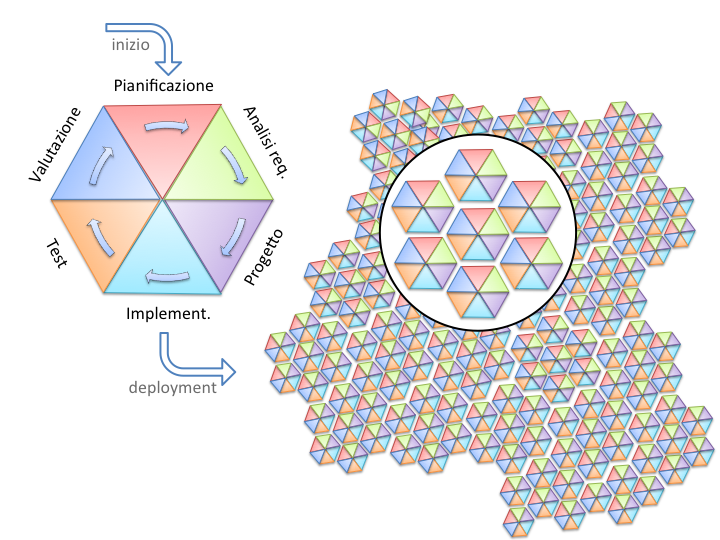
\includegraphics[scale=0.5]{img/modello_incrementale.png}
		\caption{Rappresentazione del modello incrementale\protect\footnotemark}
		\label{fig:modello_incrementale}
	\end{figure}

	\footnotetext{Fonte in \S\ref{rifinfo}}
	
    \section{Qualità di processo}\label{QualitaProcesso}

\subsection{Scopo}
La qualità di un prodotto è fortemente influenzata dal processo utilizzato nell'arco di creazione del prodotto stesso: da un tubo sporco non può uscire acqua pulita.

Per questo è necessario operare con un buon \gloss{ciclo di vita} per i processi, che devono venire verificati e valutati adeguatamente. A questo scopo viene seguito lo schema del \gloss{ciclo di Deming} e dell'\gloss{ISO 15504} descritti all'Appendice \S\ref{StandardQualita}.


\subsection{Nomenclatura metriche e obiettivi di qualità}
La nomenclatura degli obiettivi di qualità, delle \gloss{metriche} ed il loro funzionamento è spiegato in dettaglio nelle \NdP. In questa sezione gli obiettivi e le metriche vengono sinteticamente descritte:

	\begin{itemize}
		\item \textbf{Obiettivi}: 
		
		\begin{center}
			\texttt{QPR[ID] [Nome]}
		\end{center} 
		
		\begin{itemize}
			\item \textbf{QPR}: indica "Qualità di processo".
			\item \textbf{ID}: numero progressivo di tre cifre.
			\item \textbf{Nome}: descrive brevemente il processo.
		\end{itemize}
		
		\item \textbf{Metriche}:
		
		\begin{center}
			\texttt{MPR[ID] [Nome]}
		\end{center}
		
		\begin{itemize}
			\item \textbf{MPR}: indica "Metrica di processo".
			\item \textbf{ID}: numero progressivo di tre cifre.
			\item \textbf{Nome}: descrive brevemente la metrica.
		\end{itemize}
		
	\end{itemize}




\subsection{Processi}
I processi saranno elencati nel seguente modo:

\begin{center}
	\texttt{PROC[ID] [Nome]}
\end{center}

\begin{itemize}
	\item \textbf{PROC}: sta a indicare "Processo".
	\item \textbf{ID}: un numero incrementale di tre cifre per indicare in modo univoco il processo.
	\item \textbf{Nome}: una breve frase per indicare la funzione del processo.
\end{itemize}

Per ogni processo sono elencate le sue funzioni principali, gli obiettivi che \gruppo\ si prefigge per ottenere la qualità desiderata e le metriche adottate per raggiungere quell'obiettivo (quando previste).
%Gli obiettivi di qualità elencati, quando è possibile, sono affiancati da una particolare metrica. 

	\subsubsection{PROC001 Pianificazione del progetto, organizzazione e struttura}
	Tale \gloss{macro-processo} ha lo scopo di pianificare il lavoro da svolgere per soddisfare i \gloss{requisiti} richiesti dal \gloss{progetto}. È in questo processo che viene messo in atto il \gloss{way of working} del \gloss{team di sviluppo} che ha un'importanza particolare perché i suoi risultati vanno a condizionare l'esito della qualità dell'intero progetto.
	
		\paragraph*{Funzioni}
	
		\begin{itemize}
			\item \textbf{Sviluppare \gloss{sotto-processi}}: i vari obiettivi devono poter essere associati ad azioni ben precise, ognuna delle quali appartiene ad un sotto-processo.
			\item \textbf{Suddividere i compiti}: assegnazione dei compiti da realizzare ai vari componenti di \gruppo.
			\item \textbf{Candelarizzare i documenti}: stabilire delle \gloss{baseline} durante il progetto.
			\item \textbf{\gloss{Formazione} personale}: data l'inesperienza del team è richiesto un periodo di formazione personale più lungo del normale. Questo periodo deve essere contato all'interno della calendarizzazione.
			\item \textbf{Standard}: vengono scelti gli standard più convenienti da seguire.
			\item \textbf{\gloss{Budget}}: è necessario conoscere le proprie risorse in termini di tempo $\frac{\text{costo}}{\text{persona}}$ in modo tale da restare
				il più fedeli possibile al \gloss{preventivo} stilato.
		\end{itemize}
	
		\paragraph*{Metriche}
		
		\begin{itemize}
			\item MPR001 Varianza della \gloss{pianificazione}
			\item MPR002 Varianza dei costi
			\item MPR003 Aderenza agli standard
			\item MPR004 Frequenza \gloss{commit} nella \gloss{repository}
		\end{itemize}
	
		\paragraph*{Obiettivi}
		
		\begin{itemize} 
			\item \textbf{QPR001 Rispetto dei periodi della pianificazione}: all'interno della presente nel \PdPd, sono presenti le date di scadenza delle varie attività. L'obiettivo è quello di rispettarle il più possibile per proseguire al meglio la realizzazione del progetto.
			\item \textbf{QPR002 Variazione del budget}: le risorse messe a disposizione all'inizio del progetto devono potersi mantenere tali in tutta la sua durata.
			\item \textbf{QPR003 Rispetto delle fasi del ciclo di vita}: ogni processo deve rispettare le fasi del ciclo di Deming.
			\item \textbf{QPR004 \gloss{Versionamento}}: durante ogni processo, i prodotti che vengono realizzati devono possedere un numero di versione in modo da tener traccia delle modifiche. In questo modo è possibile sapere le cause di certi comportamenti dovuti ad un mutamento del prodotto in modo molto rapido. L'obiettivo è quindi tenere sotto controllo l'andamento dei cambiamenti.
		\end{itemize}
	
	\subsubsection{PROC002 Analisi}
	Il processo di analisi serve per comprendere le richieste del progetto che consistono in: requisiti, tecnologie da utilizzare e risorse da spendere.
	Insieme all'analisi dei requisiti, questo processo prevede anche l'analisi dei rischi presente alla sezione (sezione dell'analisi dei rischi) nel \Doc{\PdPv}.
	
	Completata questa attività il team di sviluppo, oltre ad aver studiato i vari requisiti, deve poter dire se il progetto risulta fattibile per le sue possibilità in termini di competenze e risorse.
	
	Tale processo non deve essere rendicontato per il preventivo a finire.
	
		\paragraph*{Funzioni}
		
		\begin{itemize}
			\item \textbf{Individuare i requisiti}: il capitolato che viene presentato dal cliente può possedere con un lessico più discorsivo che tecnico dovuto all'inesperienza del cliente nel settore.
				\`E necessario dunque effettuare un lavoro di "traduzione" per individuare i requisiti e classificarli in

			\begin{itemize}
				\item Obbligatori
				\item Desiderabili  
				\item Opzionali
			\end{itemize}
			\item \textbf{Individuare le tecnologie da utilizzare}: in base al tipo di progetto le tecnologie da utilizzare migliori per realizzarlo possono cambiare da progetto a progetto.
			\item \textbf{Comprendere la quantità di risorse richieste}: sviluppare un preventivo è fondamentale, sia per il cliente che vuole sapere il costo del progetto, che per il \gloss{fornitore} che deve sapere se il progetto per lui è fattibile.
			\item \textbf{Individuare i rischi}: lungo il corso del progetto possono accadere degli imprevisti, perciò è necessario poterli prevedere ed organizzare fin da subito una reazione ad essi.
			\item \textbf{Stabilire la fattibilità del progetto}: dopo aver fatto l'analisi dei requisiti, dei rischi e dei costi bisogna sapere se iniziare lo sviluppo del progetto o meno.
		\end{itemize}

		\paragraph*{Metriche}

		\begin{itemize}
			\item \textbf{MPR005 Requisiti obbligatori non soddisfatti}
			\item \textbf{MPR006 Requisiti desiderabili non soddisfatti}
			\item \textbf{MPR007 Requisiti opzionali non soddisfatti}
			\item \textbf{MPR008 Rischi non previsti avvenuti}
		\end{itemize}
		I risultati di tutte queste metriche possono essere pubblicate ed analizzate solo a progetto compiuto, prima avrebbe poca utilità. 
	
		\paragraph*{Obiettivi}
		
		\begin{itemize}
			\item \textbf{QPR005 Soddisfacimento dei requisiti obbligatori}: tutti i requisiti obbligatori devono essere soddisfatti a fine progetto.
			\item \textbf{QPR006 Soddisfacimento dei requisiti opzionali e desiderabili}: i requisiti opzionali e desiderabili possono non essere rispettati
				solo se non avanzano più risorse in termini di $ \frac{\text{tempo}}{\text{persona}}$ prima della consegna del progetto. I requisiti inoltre
				devono essere stabiliti in modo corretto: hanno l'obbligo di rispecchiare quanto chiesto dal cliente e non sovrapporsi tra loro.
			\item \textbf{QPR007 Verificarsi dei rischi previsti}: lo sviluppo del progetto deve essere sicuro e non presentare imprevisti la cui soluzione non è stata prevista, perché potenzialmente aumenterebbe di molto il ritardo nello sviluppo del progetto rispetto al rischio previsto.
		\end{itemize}
	
	\subsubsection{PROC003 Produzione documenti}
	Questo processo rimane attivo in tutta la durata del ciclo di vita del prodotto perché ha il compito di produrre dei documenti che riportino le scelte effettuate, gli strumenti utilizzati e le modifiche attuate nell'intero corso del progetto.
	
		\paragraph*{Funzioni}
		Il processo comprende il ciclo di vita di ogni documento, che è spiegato in dettaglio nelle \Doc{\NdPv}, prevede:
		
		\begin{itemize}
			\item Redazione
			\item Verifica
			\item Approvazione
		\end{itemize}
	
		\paragraph*{Obiettivi}
		
		\begin{itemize}
			\item \textbf{QPR008 Rispetto delle fasi del ciclo di vita}: il ciclo di vita di ogni documento deve essere rispettato in ogni sua fase e questo deve venir pubblicato secondo le scadenze stabilite. Le sue fasi sono:
			
			\begin{itemize}
				\item Redazione
				\item Verifica
				\item Approvazione
			\end{itemize}
		\end{itemize}

	\subsubsection{PROC004 Verifica}
	Il processo, attivo in tutta la durata del progetto, ha il compito di valutare la correttezza dei prodotti dati in input e stabilire se presentano errori
	e se sono sufficientemente di qualità. Il processo di verifica è descritto più nel dettaglio alla sezione §4.2 del documento \mbox{\Doc{\NdPv}}.
	
		\paragraph*{Funzioni}
		
		\begin{itemize}
			\item \textbf{Verificare le funzionalità dei prodotti}: i prodotti devono saper soddisfare i requisiti richiesti. Nella fase di verifica viene accertato che questo effettivamente avvenga.
			\item \textbf{Verificare la corretta esecuzione dei processi}: i processi possiedono un ciclo di vita che è suddiviso in fasi, per la buona esecuzione del processo queste devono essere eseguite nell'ordine corretto restituendo gli output attesi.
			\item \textbf{Verificare che siano rispettate le \NdP}: il team di sviluppo stabilisce un suo way of working che deve rispettare in tutta la durata del progetto. Anche la verifica di queste norme deve essere effettuata.
		\end{itemize}
		
		\paragraph*{Metriche}
		
		\begin{itemize}
			\item MPR009 Frequenza controllo prodotti
		\end{itemize}
		
		\paragraph*{Obiettivi}
		
		\begin{itemize}
			\item \textbf{QPR009 Effettuare una verifica costante}: la fase di verifica è sempre attiva perché ogni singolo prodotto deve essere testato e controllato ogni volta che viene modificato o prima della scadenza di una \gloss{milestone}.
			%\item \textbf{QPR010 Rispetto delle fasi di verifica}: la fase di verifica deve essere eseguita in modo iterativo senza cambiare in modo sostanziale nel corso del progetto. Un mutamento della fase di verifica renderebbe incoerenti i risultati delle precedenti iterazioni, impedendo di vedere se è presente un miglioramento della qualità o meno.
		\end{itemize}

\subsection{Tabella qualità di processo}
Le tabelle indicano gli obiettivi di qualità che ogni processo deve possedere.

Ogni obiettivo di qualità è indicato con:

\begin{itemize}
	\item \textbf{Obiettivo}: viene indicato l'obiettivo di qualità col suo codice identificativo e nome;
	\item \textbf{Metrica}: la metrica utilizzata per valutare l'obiettivo di qualità assegnatole. Nel caso non fosse possibile associare una metrica ad un obiettivo di qualità questa non verrà indicata;
	\item \textbf{Valore desiderato}: il valore che si vuole ottenere attraverso la metrica indicata per soddisfare a pieno l'obiettivo di qualità;
	\item \textbf{Descrizione}: descrizione generale dell'obiettivo di qualità e della metrica.
\end{itemize}

\newcommand{\grigiodesc}{gray!15}

\begin{table}[H]
	{\def\arraystretch{1.4}
	\begin{tabularx}{\textwidth}{YYY}
		\rowcolor{white}
		\multicolumn{3}{>{\hsize=\dimexpr3\hsize+4\tabcolsep}Y}{\textbf{PROC001 Pianificazione del progetto, organizzazione e struttura}} \\
		\rowcolor{gray!30}
		\textbf{Obiettivo} &
		\textbf{Metrica} &
		\textbf{Valore desiderato}\\\toprule
		\rowcolor{white}

		QPR001 Rispetto delle fasi dell'organigramma & MPR001 Varianza della programmazione & 0-2 giorni\\
		\rowcolor{\grigiodesc} \multicolumn{3}{>{\hsize=\dimexpr3\hsize+4\tabcolsep}X}{\textbf{Descrizione}: le scadenze date dall'organigramma possono possedere un ritardo massimo di due giorni, per le scadenza infatti viene considerato anche un tempo di \gloss{slack} per eventuali ritardi. Il valore desiderato indica la media del numero di giorni di ritardo nella chiusura di una \gloss{issue} durante tutto il macro periodo.} \\

		\hline \rowcolor{white}
		QPR002 Variazione del budget & MPR002 Varianza dei costi & \EUR{0-200}\\
		\rowcolor{\grigiodesc} \multicolumn{3}{>{\hsize=\dimexpr3\hsize+4\tabcolsep}X}{\textbf{Descrizione}: ogni ruolo nel team di sviluppo possiede una tariffa oraria. Può accadere che nel corso del progetto sia richiesto più lavoro di quello conteggiato nel preventivo, queste ore in più devono essere rendicontate.} \\
		\hline \rowcolor{white}
		QPR003 Rispetto delle fasi del ciclo di vita & MPR003 Aderenza agli standard & Livello di maturità: 3 Valutazione attributi: L\\
		\rowcolor{\grigiodesc} \multicolumn{3}{>{\hsize=\dimexpr3\hsize+4\tabcolsep}X}{\textbf{Descrizione}: dai sondaggi è emerso che la maggior parte delle aziende italiane che si sono adeguate allo standard ISO/IEC 15504 ha raggiunto un livello di maturità pari a 3. Il team di sviluppo si prefigge di raggiungere anch'esso un tale livello di maturità soddisfacendo i vari attributi di almeno il 75\% della loro interezza.}\\
		\hline \rowcolor{white}
		QPR004 Versionamento & MPR004 Frequenza commit nella repository & 25\\
		\rowcolor{\grigiodesc} \multicolumn{3}{>{\hsize=\dimexpr3\hsize+4\tabcolsep}X}{\textbf{Descrizione}: il frequente commit in una repository permette di tenere una miglior traccia delle modifiche e di accedere all'ultima versione del progetto a tutti i membri del team di sviluppo. Nel valore desiderato è indicato il numero minimo di commit da effettuare in media ogni settimana lavorativa durante il un macro periodo.}\\
	\end{tabularx}}
	\caption{Obiettivi di qualità per il PROC001}
\end{table}

\mydoublerule{\linewidth}{0pt}{2pt}

\begin{table}[H]
	{\def\arraystretch{1.4}
	\begin{tabularx}{\textwidth}{YYY}
		\rowcolor{white}
		\multicolumn{3}{>{\hsize=\dimexpr3\hsize+4\tabcolsep}Y}{\textbf{PROC002 Analisi}}\\
		\rowcolor{gray!30}
		\textbf{Obiettivo} &
		\textbf{Metrica} &
		\textbf{Valore desiderato}\\\toprule
		\rowcolor{white}
		QPR005 Soddisfacimento dei requisiti obbligatori & MPR005 Requisiti obbligatori non soddisfatti & 0\\
		\rowcolor{\grigiodesc} \multicolumn{3}{>{\hsize=\dimexpr3\hsize+4\tabcolsep}X}{\textbf{Descrizione}: i requisiti obbligatori devono essere tutti soddisfatti alla consegna finale del progetto.}\\
		\hline \rowcolor{white}
		QPR006 Soddisfacimento dei requisiti opzionali e desiderabili & MPR006 Requisiti desiderabili non soddisfatti MPR007 Requisiti opzionali non soddisfatti & 0-(n-2)\\
		\rowcolor{\grigiodesc} \multicolumn{3}{>{\hsize=\dimexpr3\hsize+4\tabcolsep}X}{\textbf{Descrizione}: i requisiti opzionali e desiderabili, non essendo
			obbligatori possono non essere svolti all'interno del progetto, dato che però offrono un valore aggiunto, il team di sviluppo vuole soddisfarne almeno due.}\\
		\hline \rowcolor{white}
		QPR007 Verificarsi dei rischi previsti & MPR008 Rischi non previsti avvenuti & 0\\
		\rowcolor{\grigiodesc} \multicolumn{3}{>{\hsize=\dimexpr3\hsize+4\tabcolsep}X}{\textbf{Descrizione}: il verificarsi di imprevisti può accadere nel corso
			del progetto, ma devono essere tutti già previsti dal team di sviluppo in modo tale da intervenire tempestivamente con una soluzione.}\\
	\end{tabularx}}
	\caption{Obiettivi di qualità per il PROC002}
\end{table}

\mydoublerule{\linewidth}{0pt}{2pt}

\begin{table}[H]
	{\def\arraystretch{1.5}
	\begin{tabularx}{\textwidth}{YYY}
		\rowcolor{white}
		\multicolumn{3}{>{\hsize=\dimexpr3\hsize+4\tabcolsep}Y}{\textbf{PROC003 Produzione documenti}}\\
		\rowcolor{gray!30}
		\textbf{Obiettivo} &
		\textbf{Metrica} &
		\textbf{Valore desiderato}\\\toprule
		\rowcolor{white}
		QPR008 Rispetto delle fasi del ciclo di vita & - & -\\
		\rowcolor{\grigiodesc} \multicolumn{3}{>{\hsize=\dimexpr3\hsize+4\tabcolsep}X}{\textbf{Descrizione}: ogni documento deve attraversare determinate fasi del ciclo di vita, è compito del \Ver~accertarsi che tali fasi vengano rispettate.}\\
	\end{tabularx}}
	\caption{Obiettivi di qualità per il PROC003}
\end{table}

\mydoublerule{\linewidth}{0pt}{2pt}

\begin{table}[H]
	{\def\arraystretch{1.5}
	\begin{tabularx}{\textwidth}{YYY}
		\rowcolor{white}
		\multicolumn{3}{>{\hsize=\dimexpr3\hsize+4\tabcolsep}Y}{\textbf{PROC004 Verifica}}\\
		\rowcolor{gray!30}
		\textbf{Obiettivo} &
		\textbf{Metrica} &
		\textbf{Valore desiderato}\\\toprule
		\rowcolor{white}
		QPR009 Effettuare una verifica costante & MPR009 Frequenza controllo prodotti & 5 modifiche\\
		\rowcolor{\grigiodesc} \multicolumn{3}{>{\hsize=\dimexpr3\hsize+4\tabcolsep}X}{\textbf{Descrizione}: il \Ver\ deve controllare i prodotti in modo frequente, in modo tale che siano corretti nella forma, contenuto e funzionalità. Per quanto riguarda i documenti le modifiche sono le varie versioni del documento riportate nel diario, per i prodotti software invece i commit effettuati.}\\
		\hline \rowcolor{white}
%		QPR010 Rispetto delle fasi di verifica & - & -\\
%		\rowcolor{\grigiodesc} \multicolumn{3}{>{\hsize=\dimexpr3\hsize+4\tabcolsep}X}{\textbf{Descrizione}: è compito del \Ver~assicurarsi che la fase di verifica venga eseguita nel modo corretto per disporre sempre di risultati di verifica attendibili ed analizzabili.}\\
	\end{tabularx}}
	\caption{Obiettivi di qualità per il PROC003}
\end{table}

\mydoublerule{\linewidth}{0pt}{2pt}
    \section{Qualità di prodotto}

\subsection{Scopo}
testo

\subsection{Prodotti}
testo

	\subsubsection{Documenti}
	testo
	
\subsection{Eventuali tabelle}
testo

\subsection{The Twelve-Factor App}
breve accenno e descrizione	    
    %\section{Sintesi delle metriche}
Contenuto
    %\section{Specifica dei test}
Contenuto

    \subsection{Tipi di test}
    Contenuto

    \subsubsection{Test di unit\`a}
    Contenuto

    \subsubsection{Test di integrazione}
    Contenuto

    \subsubsection{Test di sistema}
    Contenuto

    \subsubsection{Test di validazione}
    Contenuto

    
    \appendix
    \newpage

\section{Standard di qualità}	\label{standard di qualità}
Prendiamo come riferimento per gli obiettivi di qualità del prodotto determinati standard.


In questa appendice descriviamo gli standard adottati nelle loro parti più rilevanti ai fini del progetto. Nelle \NdPd\ viene indicato in che misura questi standard saranno applicati e nel \PdQd\ il piano che abbiamo scelto per rispettarli.

	\subsection{ISO/IEC 15504 (SPICE)}\label{iso15504}
	Lo standard ISO/IEC 15504 è stato creato per unire in un unico standard le caratteristiche principali di \gloss{CMMI} e \gloss{SPY}; entrambi standard riguardanti la qualità di processi software.
	ISO/IEC 15504 è chiamato anche SPICE come acronimo di \textit{Software Process Improvement and Capability Determination}, dando importanza al termine ``Capability'' inteso come la capacità di un processo di essere cognitivamente capace di raggiungere il suo scopo. 
	
	Un processo con un'alta Capability è osservato da tutti in modo disciplinato e sistematico.
	In caso di bassa Capability il processo viene effettuato in modo opportunistico e disorganizzato.\\
	
	SPICE mette a disposizione una metrica per valutare diversi attributi per ogni processo ed assegna un valore quantificabile ad ognuno di questi in modo tale da rendere esplicito come poter migliorare tale processo. Ogni valutazione in questo modo può essere ripetibile, oggettiva e comparabile.
	
	I processi vengono classificati in:

	

	\begin{itemize}
		\item Cliente/Fornitore
		\item Ingegneria
		\item Supporto
		\item Gestione
		\item Organizzazione
	\end{itemize}
	
	I livelli sono:
	
	\begin{itemize}
		\item \textbf{0 Incompleto}: il processo è caotico perché con risultati e performance incomplete.
	
		\item \textbf{1 Performato}: il processo inizia ad essere eseguito mettendo a disposizione degli input ed output.
		
		Attributi:
		
		\begin{itemize}
			\item \textbf{Esecuzione dei processi}: indica il numero di obiettivi raggiunti.
		\end{itemize}
	
		\item \textbf{2 Gestito}: le responsabilità e la gestione del processo sono definite.
		
		Attributi:
		
		\begin{itemize}
			\item \textbf{Gestione del processo}: indica quanto sono organizzati gli obiettivi fissati.
			\item \textbf{Gestione del prodotto}: indica quanto sono organizzati o gestiti i prodotti rilasciati.
		\end{itemize}
	
		\item \textbf{3 Stabilito}: il processo è pronto per diventare un processo standard ed essere rilasciato.
		
		Attributi:
		
		\begin{itemize}
			\item \textbf{Definizione del processo}: indica quanto il processo aderisce agli standard.
			\item \textbf{Distribuzione del processo}: indica in che misura il processo possa essere rilasciato potendo restituire sempre lo stesso risultato.
		\end{itemize}
	
		\item \textbf{4 Prevedibile}: il processo è in grado di essere sottoposto a metriche e valutazioni quantitative. Spesso i risultati sono predicibili.
		
		Attributi:
		
		\begin{itemize}
			\item \textbf{Misurazioni del processo}: indica quanto le metriche possono essere applicate al processo.
			\item \textbf{Controllo del processo}: indica quanto i risultati delle valutazioni siano predicibili.
		\end{itemize}
	
		\item \textbf{5 Ottimizzante}: il processo attua miglioramenti qualitativi e quantitativi.
		
		Attributi:
		
		\begin{itemize}
			\item \textbf{Innovazione del processo}: indica quanto i cambiamenti attuati nel processo risultino innovativi e positivi grazie ad una fase di analisi.
			\item \textbf{Ottimizzazione del processo}: indica quanto la curva di miglioramento del processo sia lineare.
		\end{itemize}
	\end{itemize}
	
	Ad ogni attributo viene data una valutazione assegnata in base alla percentuale di soddisfacimento dell'attributo:
	
	\begin{itemize}
		\item \textbf{N}: il processo non è implementato e non svolge niente di significativo (0\%-15\%).
		\item \textbf{P}: il processo è parzialmente implementato (15\%-50\%).
		\item \textbf{L}: il processo è largamente implementato (50\%-85\%).
		\item \textbf{F}: il processo è completamente implementato (85\%-100\%).
	\end{itemize}
	
\begin{table}[H]
	\centering
	\begin{oldtabular}{ccccc}
		\toprule
		\multirow{2}{*}{Attributi} & \multicolumn{4}{c}{Valutazioni}\\
		\cmidrule(lr){2-5} & N & P & L & F\\
		\midrule Esecuzione dei processi & \multicolumn{4}{c}{[0-1]}\\
		% Esecuzione dei processi & \multicolumn{4}{c}{[0-1]}\\
		\midrule Gestione del processo & \multicolumn{4}{c}{\multirow{2}{*}{[1-2]}}\\
		Gestione del prodotto\\
		\midrule Definizione del processo & \multicolumn{4}{c}{\multirow{2}{*}{[2-3]}}\\
		Distribuzione del processo\\
		\midrule Misurazione del processo & \multicolumn{4}{c}{\multirow{2}{*}{[3-4]}}\\
		Controllo del processo\\
		\midrule Innovazione del processo & \multicolumn{4}{c}{\multirow{2}{*}{[4-5]}}\\
		Ottimizzazione del processo\\
		\bottomrule
	\end{oldtabular}
	\label{tab:spice}
	\caption{Schema degli attributi di ISO/IEC 15504}
	\end{table}

%FIXME: dire a che minghie serve sta roba e quali punti in particolare
	\subsection{ISO/IEC 9126:2001}
	ISO/IEC 9126 è uno standard inerente alla qualità del software. Esso è strutturato in modo tale che si possa migliorare l'insieme dei processi.
	
	La sua struttura prevede tre tipi di qualità, ognuna delle quali possiede determinate caratteristiche:
	
	\begin{itemize}
		\item \textbf{Qualità interna}: misura la qualità di chi causa l'esecuzione del prodotto, in questo caso parliamo del codice sorgente a chi si possono assegnare diverse metriche attraverso l'analisi statica che ne stabiliscono poi la portabilità e la manutenibilità.
		
		Gli attributi ad essa assegnati sono:
		
		\begin{itemize}
			\item Manutenibilità
			\item Portabilità
		\end{itemize}
	
		\item \textbf{Qualità esterna}: misura attraverso l'analisi dinamica quanto l'esecuzione del prodotto rispetti gli obiettivi prefissati.
		
		Gli attributi ad essa assegnati sono:
		
			\begin{itemize}
			\item Funzionalità
			\item Efficienza
			\item Affidabilità
			\item Usabilità
		\end{itemize}
	
		\item \textbf{Qualità in uso}: definisce le metriche del prodotto rilasciato ed usato dal cliente che ne misurerà la qualità.
		
		Gli attributi ad essa assegnati sono:
		
		\begin{itemize}
			\item Efficacia
			\item Produttività
			\item Soddisfazione
			\item Safety
		\end{itemize}
	\end{itemize}

		\subsubsection{Descrizione degli attributi della qualità interna e della qualità esterna}
		\begin{itemize}
			\item \textbf{Manutenibilità}: il software nel corso delle sue revisioni deve essere facilmente modificabile.
			
			Nello specifico si prevede:
			
			\begin{itemize}
				\item \textbf{Analizzabilità}: prevedere una lettura del codice fruibile.
				\item \textbf{Modificabilità}: poter capire subito dove applicare la modifica.
				\item \textbf{Stabilità}: evitare effetti indesiderati dopo le modifiche.
				\item \textbf{Testabilità}: poter creare facilmente dei test su tutto il codice.
			\end{itemize}
		
			\item \textbf{Portabilità}: il software dovrebbe poter essere eseguito in più ambienti.
			
			Nello specifico si prevede:
			
			\begin{itemize}
				\item \textbf{Adattabilità}: potersi adattare automaticamente ai vari ambienti:
				\item \textbf{Installabilità}: la sua fase d'installazione dovrebbe essere semplice.
				\item \textbf{Conformità}: il software deve sapere coesistere con le altre applicazioni.
				\item \textbf{Sostituibilità}: essere capace di sostituire un software con gli stessi scopi.
			\end{itemize}
		
			\item \textbf{Funzionalità}: il software deve mettere a disposizione le funzionalità richieste in rapporto all'ambiente d'esecuzione.
			
			Nello specifico si prevede:
			
			\begin{itemize}
				\item \textbf{Appropriatezza}: le funzionalità del software sono appropriate ai requisiti richiesti.
				\item \textbf{Accuratezza}: in che misura le funzionalità aderiscono ai requisiti richiesti.
				\item \textbf{Interoperabilità}: la capacità di interagire coi sistemi specificati.
				\item \textbf{Security}: proteggere le informazioni da agenti esterni.
			\end{itemize}
		
			\item \textbf{Efficienza}: misura della capacità di raggiungere gli obiettivi stabiliti cercando di usare meno risorse possibili, in particolare:
			
			\begin{itemize}
				\item \textbf{Nel tempo}: poter dare risposte in un tempo di scadenza appropriato.
				\item \textbf{Nello spazio}: utilizzo del minor numero di risorse.
			\end{itemize}
		
			\item \textbf{Affidabilità}: il software deve mantenere le specifiche richieste senza inconvenienti.
			
			Nello specifico si prevede:
			
			\begin{itemize}
				\item \textbf{Maturità}: indica il livello minimo delle parti del prodotto che determina poi il livello di qualità dell'intero prodotto.
				\item \textbf{Robustezza}: la capacità di saper reagire agli errori.
				\item \textbf{Recuperabilità}: per poter tornare alla versione precedente del software in modo semplice.
			\end{itemize}
		
			\item \textbf{Usabilità}: il software deve poter essere compreso fin da subito, dunque semplice ed immediato nell'utilizzo e comprensione.
			
			Nello specifico si prevede:
			
			\begin{itemize}
				\item \textbf{Comprensibilità}: il significato delle funzionalità deve essere compreso il prima possibile dall'utente.
				\item \textbf{Apprendibilità}: capacità di saper usare le funzionalità disponibili.
				\item \textbf{Operabilità}: capacità dell'utente di usare e controllare il software.
				\item \textbf{Attrattiva}: il risultato deve risultare attraente all'utente.
			\end{itemize}
		\end{itemize}
	
		\subsubsection{Descrizione degli attributi della qualità in uso}
		\begin{itemize}
			\item \textbf{Efficacia}: misura della capacità di riuscire a raggiungere i compiti fissati. Essa si calcola
			in base al grado di raggiungimento degli obiettivi.
			\item \textbf{Produttività}: intesa come $ \frac{\text{unità di prodotto realizzato}}{\text{unità di risorse utilizzate}} $.
			\item \textbf{Soddisfazione}: il software deve soddisfare l'utente.
			\item \textbf{Safety}: il software deve possedere adeguati livelli di sicurezza per il tipo di utente che ne usufruisce.
		\end{itemize}
	
	\begin{figure}[H]
		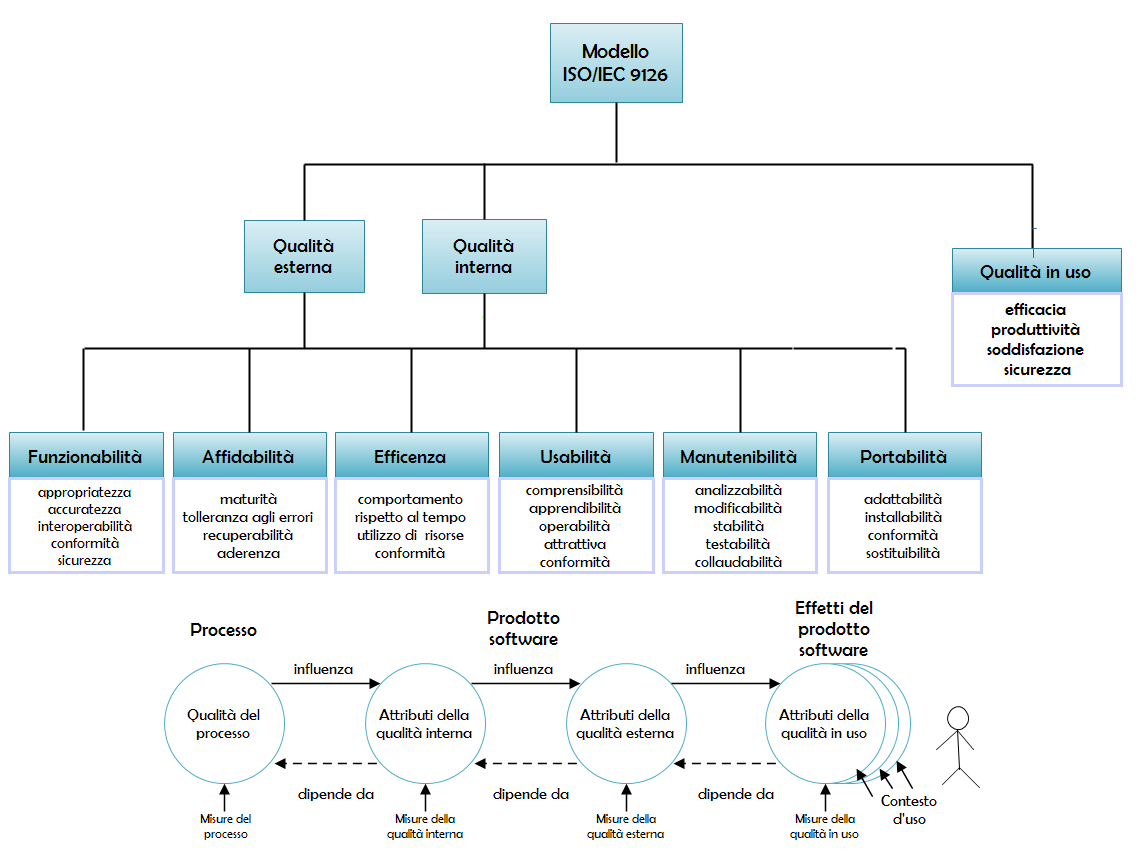
\includegraphics[width=\textwidth]{img/ISO9126_full.png}
		\label{fig:iso9126}
		\caption[Schema ISO 9126 con il suo ciclo di vita]{Schema ISO 9126 con il suo ciclo di vita\protect\footnotemark}
	\end{figure}

	\footnotetext{Vedere in \S\ref{riferimenti informativi}}
	
	\subsection{Ciclo di Deming}	\label{cicloDeming}
	Il Ciclo di Deming è un metodo iterativo creato per migliorare la qualità dei processi e dei prodotti software. È un metodo che opera nell'ottica di un miglioramento continuo in termini di risultati e risorse utilizzate e al termine di ogni ciclo, l'eventuale miglioramento effettuato diventa la nuova base da cui inizia l'iterazione successiva.
	
	Si distingue in quattro fasi, chiamate anche PDCA, che sono:
	
	\begin{itemize}
		\item \textbf{Plan}: pianificare i processi per ottenere i risultati attesi ed osservare dove questi possono essere migliorati.
		\item \textbf{Do}: eseguire il programma e i miglioramenti inseriti nella fase precedente.
		\item \textbf{Check}: effettuare test e controlli dell'output della fase precedente confrontandoli con gli obiettivi della fase di Plan. Dare una valutazione dei risultati per verificare se i cambiamenti attuati portano effettivamente dei miglioramenti.
		\item \textbf{Act}: le modifiche, se risultano essere delle migliorie vengono applicate al processo o al prodotto.
	\end{itemize}

	\begin{figure}[H]
		\centering
		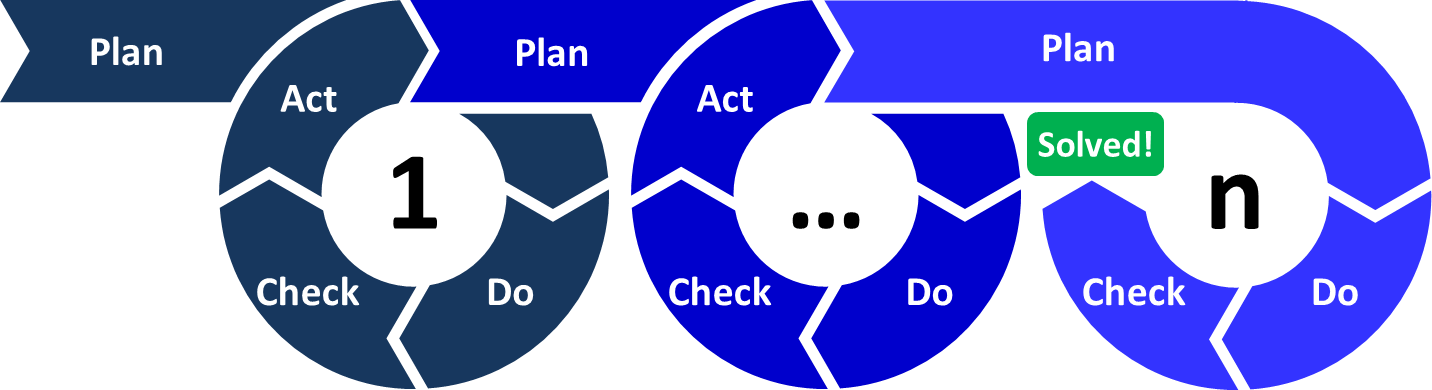
\includegraphics[width=0.65\textwidth]{img/PDCA}
		\label{fig:PDCA}
		\caption[Ciclo di Deming]{Ciclo di Deming\protect\footnotemark}
	\end{figure}

	\footnotetext{Vedere Riferimenti Informativi in \S\ref{riferimenti informativi}}

	\subsection{ISO/IEC 90003:2004}
	Lo standard ISO/IEC 90003 consiste nello standard ISO 9001:2008 applicato al software. Quest'ultimo tratta di uno standard sulla qualità dei sistemi aziendali che segue il sistema il Ciclo di Deming descritto in \S\ref{cicloDeming}.
	
	L'ISO/IEC 90003:2004 si suddivide in otto capitoli che sono:
	
	\begin{enumerate}
		\item Scopo
		\item Riferimenti normativi
		\item Termini e definizioni
		\item Sistema di gestione della qualità
		\item Gestione delle responsabilità
		\item Gestione delle risorse
		\item Realizzazione del prodotto
		\item Misurazione, analisi e miglioramento
	\end{enumerate}

	Date le nostre capacità e la nostra esperienza, prendiamo in considerazione solo alcuni punti del quarto capitolo. In particolar modo quelli riguardanti la documentazione, non potendo ancora stabilire metriche sul software.
	
	\subsubsection{Capitolo 4. dell'ISO 90003: requisiti di sistema e linee guida}
	
	\begin{enumerate}
		\item \textbf{Requisiti e linee guida sull'organizzazione}:
		\begin{enumerate}
			\item \textbf{Stabilire la gestione del sistema di qualità (QMS)}
			\begin{itemize}
				\item \textbf{Identificare i requisiti di cui il QMS ha bisogno}: attraverso il \PdQ~osservando i processi interni ed esterni.
				\item \textbf{Assicurarsi che ogni processo sia efficacie}: attraverso una verifica continua sui processi e prodotti.
			\end{itemize}
			\item \textbf{Documentare il proprio QMS}: riportare le relazioni tra i vari processi e come essi vengano gestiti e verificati.
			\item \textbf{Cercare di migliorare il proprio QMS}: applicando il ciclo di Deming.
			\item Mantenere la qualità del QMS
		\end{enumerate} 
		
		\item \textbf{Requisiti e linee guida sulla documentazione}:
		\begin{enumerate}
			\item \textbf{Documentare la qualità}:
			\begin{itemize}
				\item \textbf{Pianificare la documentazione del QMS}: assicurandosi che quello che verrà scritto rispecchi gli obiettivi e la gestione dei processi.
				\item \textbf{Stabilire la documentazione del QMS}: stabilendo la qualità delle diverse parti del QMS.
				\item Mantenere la documentazione nel tempo
			\end{itemize}
			
			\item \textbf{Controllare la qualità dei documenti}:
			\begin{itemize}
				\item \textbf{Stabilire una procedura per controllare i documenti}: documentare la stessa procedura di controllo che dovrebbe contenere la fase di approvazione del documento, un suo versionamento e continuo aggiornamento.
				\item Mantenere ed aggiornare la procedura di controllo del documento
			\end{itemize}
		\end{enumerate}
	\end{enumerate}

    \newpage

\section{Resoconto delle attività di verifica} \label{ResocontoAttivitaVerifica}
In questa sezione viene riportata una sintesi conclusiva dei risultati ottenuti dalle fasi di verifica effettuate nei vari periodi del progetto attraverso le metriche indicate in tale documento. Essi possono coincidere o meno con i valori desiderati da AlphaSix e, nel secondo caso in particolar modo, saranno oggetto di valutazioni per il miglioramento descritte all'appendice \S\ref{mitigazione variazioni}.

I test che vengono introdotti nel corso del progetto non vanno a sostituire i test precedentemente sviluppati. Ogni test, appena è creato viene eseguito periodicamente fino alla fine del progetto, per evitare che i nuovi cambiamenti possano reintrodurre errori precedentemente risolti.

	\subsection{Classificazione dei risultati} \label{classificazionerisultati}
	I risultati ottenuti tramite una metrica, rispetto all'obiettivo che vogliamo raggiungere e ai valori da noi desiderati, sono classificati in:
    
    \begin{itemize}
    	\item \textbf{Soddisfacente}: il risultato è quello atteso.
    	\item \textbf{Poco soddisfacente}: il risultato non è quello atteso, ma gli è vicino.
    	\item \textbf{Insoddisfacente}: il risultato non è per niente quello atteso.
    \end{itemize} 

	\subsection{Primo periodo (RR)}\label{ResocontoAttivitaVerifica:RP}
	Periodo individuato come \AdR\ che dura circa un mese di tempo e un quarto del tempo complessivo per realizzare il progetto.

    \subsubsection{Riassunto delle attività di verifica}
    L'attività di verifica si è rivelata per noi più faticosa del previsto. I motivi sono molteplici:
    	\begin{itemize}
    		\item Nel primo periodo perché non avevamo sufficiente esperienza per effettuare una verifica sistematica e perché la nostra attenzione si è interamente concentrata sull'organizzazione dei ruoli e la loro funzione
    		\item Nel secondo periodo invece la verifica è stata più sistematica e meno impegnativa perché gli elaborati venivano consegnati in orario, ma comunque la correzione si è rivelata onerosa
    	\end{itemize}
    

    Come indicato nelle \NdPd, l'attività di verifica è stata effettuata inizialmente attraverso Walkthrought e successivamente attraverso Inspection. Essendo ancora alle prime armi all'inizio del progetto, abbiamo effettuato la verifica secondo Walkthrough per una buona parte del periodo di analisi dei requisiti realizzata insieme. Dopodiché siamo passati ad adottare Inspection in quanto una ricerca dispersiva non era utile alla parallelizzazione dei compiti. 
    Nel momento in cui sarà necessario verificare prodotti software, riteniamo opportuno effettuare il passaggio da Walkthrough a Inspection in tempi più rapidi rispetto a come è avvenuto finora.
    
    \subsubsection{Risultati delle verifiche tramite analisi}
    Nelle tabelle seguenti vengono riportati i risultati ottenuti applicando le metriche in correlazione all'obiettivo scelto. 
    In ogni tabella sono indicati i prodotti o i processi sottoposti alle metriche e i risultati ottenuti sono presenti in ``Valutazione'', classificati secondo \S\ref{classificazionerisultati}.

    \paragraph{Documenti}

    \begin{table}[H]
    	{\def\arraystretch{1.5}
   		\begin{tabularx}{\textwidth}{YYY}
   			\rowcolor{white}
   			\textbf{QPD001 Leggibilità del testo} & \textbf{MPD001 Indice Gulpease} & \textbf{50 - 60} \\
			\hline
   			\rowcolor{gray!30}
   			\textbf{Prodotto/processo testato} & \textbf{Risultato ottenuto} & \textbf{Valutazione} \\
   			\toprule
   			\rowcolor{white} 	\NdPd & 54.57 & Soddisfacente \\
   			\rowcolor{\grigiodesc} 		\SdFd & 53.7 & Soddisfacente \\
   			\rowcolor{white} 	\PdPd & 51.75 & Soddisfacente \\
   			\rowcolor{\grigiodesc} 	\PdQd & 53.29 & Soddisfacente \\
   			\rowcolor{white} \AdRd & 55.62 & Soddisfacente \\
   			\toprule %\rowcolor{gray!30}
   			\multicolumn{3}{>{\hsize=\dimexpr3\hsize+4\tabcolsep}Y}{\textbf{Nota}: tutti i documenti soddisfano pienamente l'obiettivo di qualifica indicato.} \\ 
   		\end{tabularx}}
   	\caption{Risultati di MPD001 Indice Gulpease}
    \end{table}

	\mydoublerule{\linewidth}{0pt}{2pt}

	\begin{table}[H]
		{\def\arraystretch{1.5}
		\begin{tabularx}{\textwidth}{YYY}
			\rowcolor{white}
			\textbf{QPD002 Correttezza ortografica} & \textbf{MPD002 Correttezza
				ortografica} & \textbf{0} \\
			\hline
			\rowcolor{gray!30}
			\textbf{Prodotto/processo testato} & \textbf{Risultato ottenuto} & \textbf{Valutazione} \\
			\toprule
			\rowcolor{white} \NdPd & 0 & Soddisfacente \\
			\rowcolor{\grigiodesc} \SdFd & 0 & Soddisfacente \\
			\rowcolor{white} \PdPd & 0 & Soddisfacente \\
			\rowcolor{\grigiodesc} \PdQd & 0 & Soddisfacente \\
			\rowcolor{white} \AdRd & 0 & Soddisfacente \\
			\bottomrule
			\multicolumn{3}{>{\hsize=\dimexpr3\hsize+4\tabcolsep}Y}{\textbf{Nota}: tutti i documenti soddisfano pienamente l'obiettivo di qualifica indicato.} \\
		\end{tabularx}}
	\caption{Risultati di MPD002 Correttezza
		ortografica}
	\end{table}

	\paragraph{Processi}

		
		\begin{table}[H]
			{\def\arraystretch{1.5}
				\begin{tabularx}{\textwidth}{YYY}
					\rowcolor{white}
					\textbf{QPR001 Rispetto dei periodi della pianificazione} & \textbf{MPR001 Varianza della pianificazione} & \textbf{96 ore} \\
					\hline
					\rowcolor{gray!30}
					\textbf{Prodotto/processo testato} & \textbf{Risultato ottenuto} & \textbf{Valutazione} \\
					\toprule
					\rowcolor{white} \PdP & 7 & Soddisfacente \\
					\toprule
					\multicolumn{3}{>{\hsize=\dimexpr3\hsize+4\tabcolsep}Y}{\textbf{Nota}: non tutte le scadenze sono state rispettate, ma i ritardi sono rientrati nei valori tollerati. Il valore ottenuto è la somma delle ore di variazione dei vari ruoli.} \\
			\end{tabularx}}
			\caption{Risultati di MPR001 Varianza della pianificazione}
		\end{table}
	
		% \vspace{5pt}
		\mydoublerule{\linewidth}{0pt}{2pt}
		\vspace{20pt}
	
		\begin{table}[H]
			{\def\arraystretch{1.5}
				\begin{tabularx}{\textwidth}{YYY}
					\rowcolor{white}
					\textbf{QPR002 Variazione del budget} & \textbf{MPR002 Varianza dei costi} & \textbf{\EUR{0 - 200}} \\
					\hline
					\rowcolor{gray!30}
					\textbf{Prodotto/processo testato} & \textbf{Risultato ottenuto} & \textbf{Valutazione} \\
					\toprule\rowcolor{white}
					Differenza consuntivo rimanente e consuntivo di periodo & \EUR{ - 15,00} & Soddisfacente \\ 
					\bottomrule
					\multicolumn{3}{>{\hsize=\dimexpr3\hsize+4\tabcolsep}Y}{\textbf{Nota}: il valore desiderato indicato precedentemente sembra essere fin troppo permissivo. Il dettaglio del risultato ottenuto è indicato nel consuntivo di periodo.} \\
			\end{tabularx}}
			\caption{Risultati di MPR002 Varianza dei costi}
		\end{table}
	
		\mydoublerule{\linewidth}{0pt}{2pt}
		\vspace{20pt}
	
		\begin{table}[H]
			{\def\arraystretch{1.5}
				\begin{tabularx}{\textwidth}{YYY}
					\rowcolor{white}
					\textbf{QPR003 Rispetto delle fasi del ciclo di vita} & \textbf{MPR003 Aderenza agli standard} & \textbf{Livello di maturità: 3 Valutazione attributi: L} \\
					\hline
					\rowcolor{gray!30}
					\textbf{Prodotto/processo testato} & \textbf{Risultato ottenuto} & \textbf{Valutazione} \\
					\toprule\rowcolor{white}
					PROC001 Pianificazione del progetto, organizzazione e struttura & Livello di maturità: 2 Valutazione attributi: L & Poco soddisfacente \\
					\bottomrule
					\multicolumn{3}{>{\hsize=\dimexpr3\hsize+4\tabcolsep}Y}{\textbf{Nota}: essendo il primo periodo è prevedibile che il livello di maturità desiderato non sia ancora quello sperato. Si prevede un miglioramento per le successive revisioni.} \\
			\end{tabularx}}
			\caption{Risultati di MPR003 Aderenza agli standard}
		\end{table}
	
		%\mydoublerule{\linewidth}{0pt}{2pt}
		\vspace{20pt}
		
		\begin{table}[H]
			{\def\arraystretch{1.5}
				\begin{tabularx}{\textwidth}{YYY}
					\rowcolor{white}
					\textbf{QPR004 Versionamento} & \textbf{MPR004 Frequenza commit nella repository} & \textbf{25} \\
					\hline
					\rowcolor{gray!30}
					\textbf{Prodotto/processo testato} & \textbf{Risultato ottenuto} & \textbf{Valutazione} \\
					\toprule\rowcolor{white}
					Repository & 31.25 & Soddisfacente \\
					\bottomrule
					\multicolumn{3}{>{\hsize=\dimexpr3\hsize+4\tabcolsep}Y}{\textbf{Nota}: il numero di commit effettuati risulta ottimo.} \\
			\end{tabularx}}
			\caption{Risultati di MPR004 Frequenza commit nella repository}
		\end{table}
		
		\mydoublerule{\linewidth}{0pt}{2pt}
		\vspace{20pt}
		
		\begin{table}[H]
			{\def\arraystretch{1.5}
				\begin{tabularx}{\textwidth}{YYY}
					\rowcolor{white}
					\textbf{QPR009 Effettuare una verifica costante} & \textbf{MPR009 Frequenza controllo prodotti} & \textbf{5 Modifiche} \\
					\hline
					\rowcolor{gray!30}
					\textbf{Prodotto/processo testato} & \textbf{Risultato ottenuto} & \textbf{Valutazione} \\
					\toprule\rowcolor{white}
					Documenti & 7.2 & Poco soddisfacente \\
					\bottomrule
					\multicolumn{3}{>{\hsize=\dimexpr3\hsize+4\tabcolsep}Y}{\textbf{Nota}: il valore ottenuto non soddisfa il risultato atteso perché nella prima parte del macro periodo \gruppo\ ha prestato molta attenzione alla formazione personale a discapito del tempo che poteva essere dedicato alla verifica dei prodotti.} \\
			\end{tabularx}}
			\caption{Risultati di MPR009 Frequenza controllo prodotti}
		\end{table}
	
	%\mydoublerule{\linewidth}{0pt}{2pt}
	
	\subsection{Secondo periodo (RP)}
	Periodo individuato come Revisione Progettuale la quale dura all'incirca un mese ed un quarto dell'intera durata del progetto.
	
	\subsubsection{Riassunto delle attività di verifica}
	In questo periodo di tempo abbiamo per lo più attuato verifiche sui documenti, come per il periodo di \RR, ma in maniera più approfondita e  sistematica, e verifiche sul software, in particolare sul codice scritto per il \gloss{Proof of Concept}.

	
	\subsubsection{Risultati delle verifiche tramite analisi}
	In questa sezione riportiamo i diagrammi contenenti tutti i valori di nostro interesse per dare un giudizio sul lavoro svolto fino alla fine di questo periodo.
	Essi contengono i valori ottenuti nel tempo partendo dall'ultima consegna dei documenti (il 2019-01-14) e mostrano con chiarezza l'andamento delle misurazioni che abbiamo effettuato.
	Per questo motivo, ogni diagramma è intitolato con la metrica utilizzata ed è accompagnato da:
	\begin{itemize}
		\item \textbf{Obiettivo}: codice dell'obiettivo di qualità.
		\item \textbf{Valore desiderato}: il valore desiderato ottenibile da una determinata metrica.
		\item \textbf{Descrizione}: breve descrizione del diagramma.
		\item \textbf{Valutazione}: la nostra valutazione classificata secondo \S\ref{classificazionerisultati}.
		\item \textbf{Considerazioni}: nostro commento in relazione ai risultati ottenuti dalla misurazione.
	\end{itemize}


	\paragraph{Documenti}

	\subparagraph{MPD001 Indice di Gulpease}

	\begin{figure}[H]
		\centering
		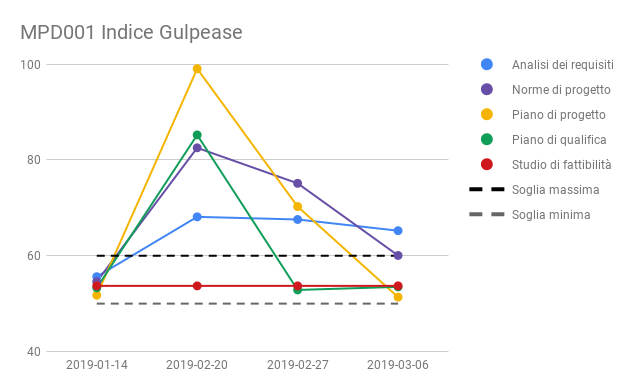
\includegraphics[width=0.9\textwidth]{img/cruscotti/MPD001.png}
		\label{immaginegulpease}
		\caption{Diagramma con valori misurati tramite MPD001 Indice di Gulpease}
	\end{figure}

	\begin{itemize}
		\item \textbf{Obiettivo}: QPD001 Leggibilità del testo.
		\item \textbf{Valore desiderato}: 50 - 60.
		\item \textbf{Descrizione}: vengono mostrati i cambiamenti dei valori dell'Indice di Gulpease nei documenti e la soglia minima e massima (in grigio e nero) in cui devono rientrare i valori dei documenti. 
		\item \textbf{Valutazione}: soddisfacente.
		\item \textbf{Considerazioni}: ogni documento ha degli alti e bassi nel corso della stesura, ma infine tutti, eccetto l'\AdR, rispettano i valori desiderati.
	\end{itemize}


	\subparagraph{MPD002 Correttezza ortografica}

	\begin{figure}[H]
		\centering
		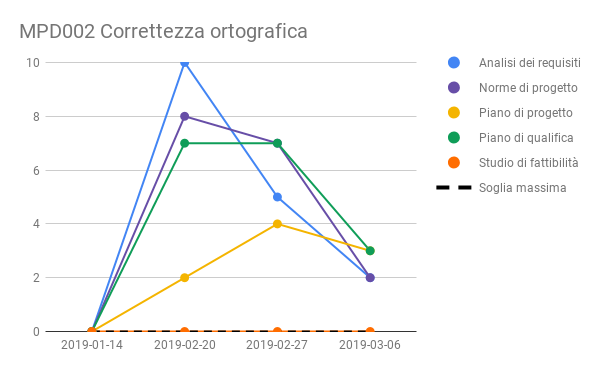
\includegraphics[width=0.9\textwidth]{img/cruscotti/MPD002.png}
		\label{immagineCorrettezzaOrtografica}
		\caption{Diagramma con valori misurati tramite MPD002 Correttezza ortografica}
	\end{figure}

	\begin{itemize}
		\item \textbf{Obiettivo}: QPD002 Correttezza ortografica.
		\item \textbf{Valore desiderato}: 0.
		\item \textbf{Descrizione}: per ogni documento è mostrato l'andamento del numero di errori ortografici e la soglia (in nero) messa a zero.
		\item \textbf{Valutazione}: soddisfacente.
		\item \textbf{Considerazioni}: dopo la modifica iniziale dei documenti il numero di errori è diminuito, tendendo ad annullarsi per la fine del periodo \RP.
	\end{itemize}



	\paragraph{Processi}

	\subparagraph{MPR001 Varianza della pianificazione}

	\begin{figure}[H]
		\centering
		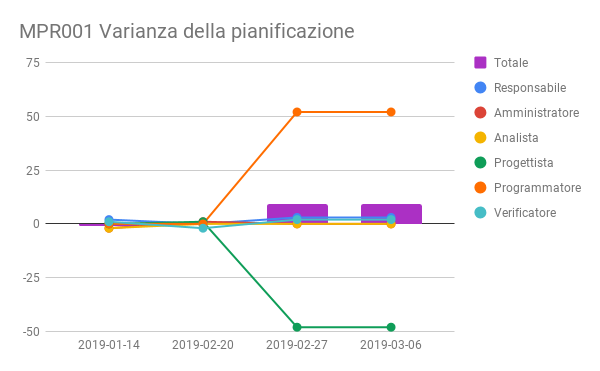
\includegraphics[width=0.9\textwidth]{img/cruscotti/MPR001.png}
		\label{immagineVarianzaPianificazione}
		\caption{Diagramma con valori misurati tramite MPR001 Varianza della pianificazione}
	\end{figure}

	\begin{itemize}
		\item \textbf{Obiettivo}: QPR001 Rispetto dei periodi della pianificazione.
		\item \textbf{Valore desiderato}: 96 ore.
		\item \textbf{Descrizione}: oltre a mostrare le ore di varianza di ogni ruolo, viene mostrato anche il totale delle ore di variazione (in viola) coi relativi valori. 
		\item \textbf{Valutazione}: poco soddisfacente.
		\item \textbf{Considerazioni}:Nelle ultime settimane siamo stati costretti a ridurre drasticamente le ore al \Prog\ per darne al \Progr\ essendo a ridosso della consegna del Proof of Concept. Questo purtroppo ha portato ad una variazione troppo elevata del preventivo in termini di ore.
	\end{itemize}


	\subparagraph{MPR002 Varianza dei costi}

	\begin{figure}[H]
		\centering
		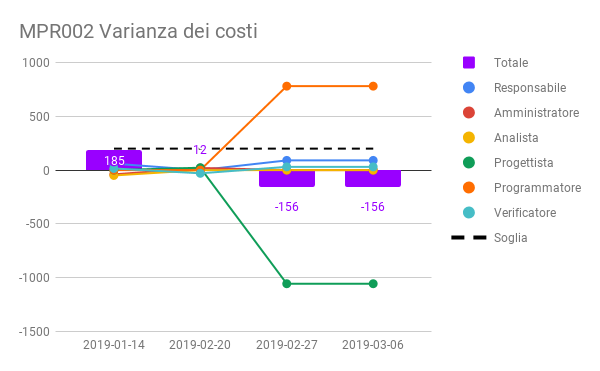
\includegraphics[width=0.9\textwidth]{img/cruscotti/MPR002.png}
		\label{immagineVarianzaCosti}
		\caption{Diagramma con valori misurati tramite MPR002 Varianza dei costi}
	\end{figure}

	\begin{itemize}
		\item \textbf{Obiettivo}: QPR002 Varianza del budget.
		\item \textbf{Valore desiderato}: \EUR{0 - 200}.
		\item \textbf{Descrizione}: vengono mostrate le variazioni della spesa attribuita ad ogni ruolo, inoltre ne viene mostrato il totale attraverso delle colonne (in viola) coi relativi valori.
		\item \textbf{Valutazione}: soddisfacente.
		\item \textbf{Considerazioni}: la diminuzione delle ore assegnate al \Prog\ a favore di quelle per il \Progr, ha portato ad una diminuzione di \EUR{156} del preventivo, un dato che comunque risulta essere soddisfacente.
	\end{itemize}
	

	\subparagraph{MPR003 Aderenza agli standard}

	\begin{figure}[H]
		\centering
		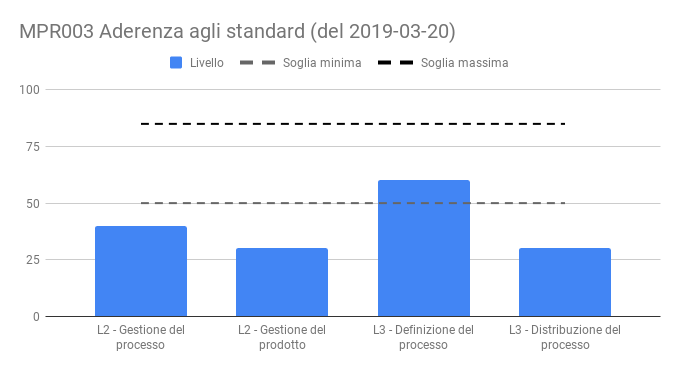
\includegraphics[width=0.9\textwidth]{img/cruscotti/MPR003_(1).png}
		\label{immagineAderenzaStandard1}
		\caption{Diagramma con valori misurati tramite MPR003 Aderenza agli standard (1)}
	\end{figure}

    \begin{figure}[H]
        \centering
        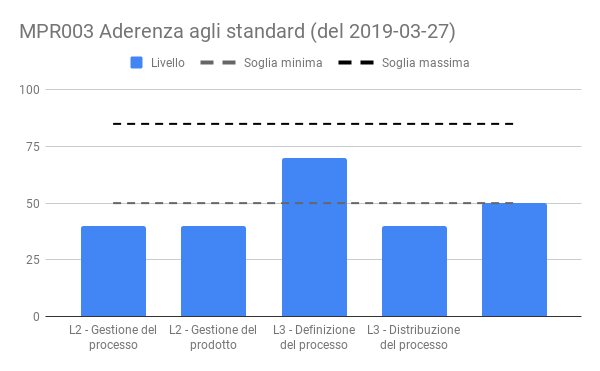
\includegraphics[width=0.9\textwidth]{img/cruscotti/MPR003_(2).png}
        \label{immagineAderenzaStandard2}
        \caption{Diagramma con valori misurati tramite MPR003 Aderenza agli standard (2)}
    \end{figure}
    
    \begin{figure}[H]
        \centering
        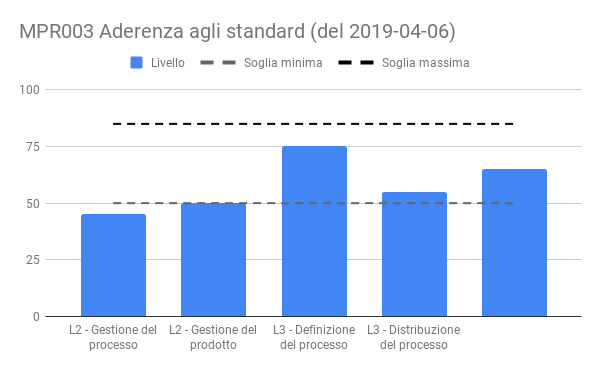
\includegraphics[width=0.9\textwidth]{img/cruscotti/MPR003_(3).png}
        \label{immagineAderenzaStandard3}
        \caption{Diagramma con valori misurati tramite MPR003 Aderenza agli standard (3)}
    \end{figure}

	\begin{itemize}
		\item \textbf{Obiettivo}: QPR003 Rispetto delle fasi del ciclo di vita.
		\item \textbf{Valore desiderato}: Livello di maturità: 3, Valutazione attributi: L.
		\item \textbf{Descrizione}: per ogni attributo dei processi viene mostrato in che percentuale sono soddisfatti attraverso le colonne (in blu), mostrando anche la soglia minima e massima (in grigio e nero) che questi valori dovrebbero avere.
		\item \textbf{Valutazione}: poco soddisfacente.
		\item \textbf{Considerazioni}: il miglioramento per quanto riguarda l'aderenza agli standard è presente, ma non ancora sufficiente per gli obiettivi prefissati.
	\end{itemize}
	



	\paragraph{Software}

	\subparagraph{MPS001 Presenza di bug}
    
    \begin{figure}[H]
        \centering
        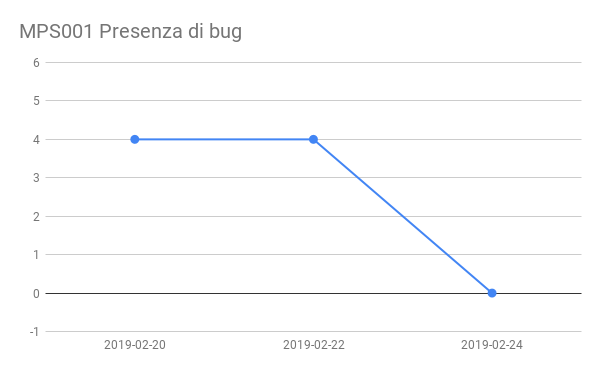
\includegraphics[width=0.9\textwidth]{img/cruscotti/MPS001.png}
        \label{immaginePresenzaBug}
        \caption{Diagramma con valori misurati tramite MPS001 Presenza di bug}
    \end{figure}
    
    \begin{itemize}
        \item \textbf{Obiettivo}: QPS001 Assenza di bug.
        \item \textbf{Valore desiderato}: 0.
        \item \textbf{Descrizione}: viene mostrato il numero totale di bug rilevati da SonarQube.
        \item \textbf{Valutazione}: soddisfacente.
        \item \textbf{Considerazioni}: per la consegna del Proof of Concept abbiamo cercato di togliere tutti i bug presenti nel codice.
    \end{itemize}

    \subparagraph{MPS002 Presenza di vulnerabilità}
    
    \begin{figure}[H]
        \centering
        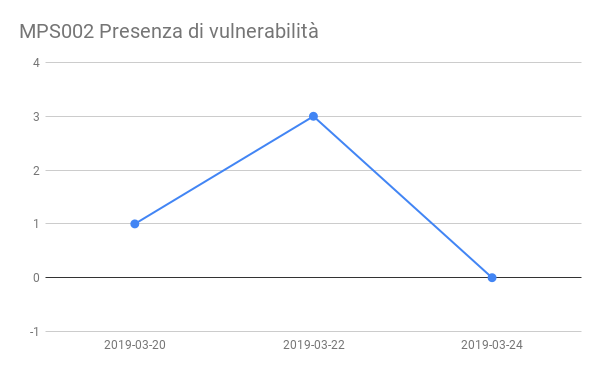
\includegraphics[width=0.9\textwidth]{img/cruscotti/MPS002.png}
        \label{immaginePresenzaVulnerabilità}
        \caption{Diagramma con valori misurati tramite MPS002 Presenza di vulnerabilità}
    \end{figure}
    
    \begin{itemize}
        \item \textbf{Obiettivo}: QPS002 Assenza di vulnerabilità.
        \item \textbf{Valore desiderato}: 0.
        \item \textbf{Descrizione}: viene mostrato il numero totale di vulnerabilità rilevate da SonarQube.
        \item \textbf{Valutazione}: soddisfacente.
        \item \textbf{Considerazioni}: per la consegna del Proof of Concept abbiamo cercato di togliere tutte le vulnerabilità presenti nel codice.
    \end{itemize}

    \subparagraph{MPS003 Presenza di code smell}
    
    \begin{figure}[H]
        \centering
        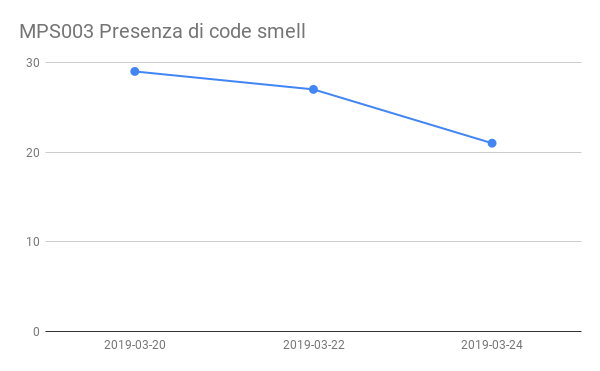
\includegraphics[width=0.9\textwidth]{img/cruscotti/MPS003.png}
        \label{immaginePresenzaCodeSmell}
        \caption{Diagramma con valori misurati tramite MPS003 Presenza di code smell}
    \end{figure}
    
    \begin{itemize}
        \item \textbf{Obiettivo}: QPS003 Assenza di code smell.
        \item \textbf{Valore desiderato}: 0.
        \item \textbf{Descrizione}: viene mostrato il numero totale di code smell rilevati da SonarQube.
        \item \textbf{Valutazione}: poco soddisfacente.
        \item \textbf{Considerazioni}: dato che non risultano essere errori particolarmente gravi all'interno del codice si ha dato priorità a correggere altri tipi di errori prima della consegna del Proof of Concept. Prevediamo di toglierli completamente nelle parti utilizzeremo successivamente per il prodotto finale.
    \end{itemize}

    \subparagraph{MPS004 Duplicazione del codice}
    
    \begin{figure}[H]
        \centering
        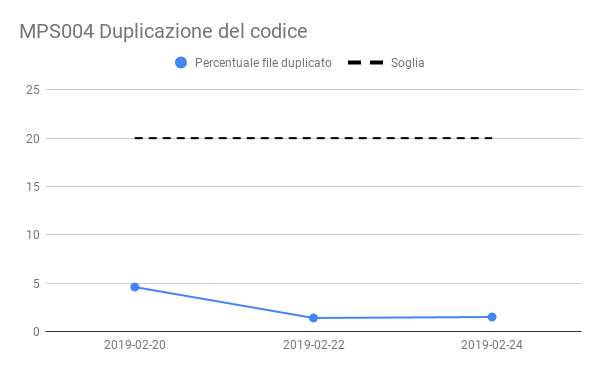
\includegraphics[width=0.9\textwidth]{img/cruscotti/MPS004.png}
        \label{immaginePresenzaDupplicazioneCodice}
        \caption{Diagramma con valori misurati tramite MPS004 Duplicazione del codice}
    \end{figure}
    
    \begin{itemize}
        \item \textbf{Obiettivo}: QPS004 Minima duplicazione del codice.
        \item \textbf{Valore desiderato}: 0 - 20\%.
        \item \textbf{Descrizione}: viene mostrata la percentuale di codice duplicato rilevato da SonarQube.
        \item \textbf{Valutazione}: soddisfacente.
        \item \textbf{Considerazioni}: La quantità di codice duplicato, dopo la prima verifica, è rimasto molto basso. Miriamo ad abbassarlo ulteriormente nel prossimo periodo, ma di non raggiungere ad un totale 0\%.
    \end{itemize}
    \newpage

\section{Consuntivo di periodo}	
	
	\subsection{Analisi dei Requisiti}
	Vengono riportate in seguito le ore di lavoro effettive relative al periodo di Analisi dei Requisiti.
	
	\begin{table}[H]
		\begin{detailtable}{\columnwidth}{m{3cm}YYYYYYY}
			\thead{Membro} & 
			\thead{Re} &
			\thead{Am} &
			\thead{An} &
			\thead{Pj} &
			\thead{Pr} &
			\thead{Ve} &
			\thead{Totale}\\\toprule\rowcolor{\tablegray}
			Ciprian Voinea & 11 (+3) & & 7 (-2) & & & 5 (-2) & 23 (-1)\\
			Laura Cameran & & 8 & 9 & & & 7 & 24\\\rowcolor{\tablegray}
			Matteo Marchiori & 7 (-1) & & 9 & & & 8 (+1) & 24\\
			Nicola Carlesso & 8 & & 10 (+1) & & & 7 & 25 (+1)\\\rowcolor{\tablegray} 
			Samuele Gardin & & 7 (-1) & 9 & & & 7 & 23 (-1)\\ 
			Timoty Graziero & & 7 (-1) & 8 (-1) & & & 9 (+2) & 24\\\bottomrule
		\end{detailtable}
		\caption{Tabella con le ore consuntivate nel periodo di Analisi dei Rischi}
	\end{table}
	
	Viene riportato in seguito il consuntivo relativo al periodo di Analisi dei Requisiti:
	
	\begin{table}[H]
		\begin{detailtable}{\columnwidth}{m{3cm}YY}
			\thead{Ruolo} & 
			\thead{Totale ore} &
			\thead{Costo in \euro}\\\toprule\rowcolor{\tablegray}
			Responsabile & 26 (+2) & 780,00 (+60,00)\\
			Amministratore & 22 (-2) & 440,00 (-40,00)\\\rowcolor{\tablegray}
			Analista & 52 (-2) & 1300,00 (-50,00)\\
			Progettista & & \\\rowcolor{\tablegray}
			Programmatore & &\\
			Verificatore & 43 (+1) & 645,00 (+15,00)\\\rowcolor{\tablegray}
			Totale & 143 (-1) & 3165,00 (-15,00)\\\bottomrule
		\end{detailtable}
		\caption{Tabella con il consuntivo del periodo di Analisi dei Rischi}
	\end{table}
	
	\subsection{Conclusioni}
	Non si ritiene opportuno aggiungere osservazioni in merito al discostamenti di orario rispetto a quanto preventivato.\\
	Questo primo consuntivo di periodo è di utilità per \gruppo\ di modo da poter osservare in modo oggettivo l'andamento del lavoro.\\
	Inoltre il preventivo iniziale viene presentato con questa prima versione del documento al proponente.
	
    \newpage
\section{Valutazioni per il miglioramento}
	
	Questo paragrafo vuole elencare i problemi riscontrati nel corso del progetto evidenziati dalle considerazioni dei vari membri di AlphaSix e dai risultati riportati all'appendice §B.
	
	Per ogni problema verrà considerata una soluzione di miglioramento da applicare dalla versione attuale del documento in avanti.

	\subsection{Valutazioni sull'organizzazione}
		\begin{itemize}
			\item \textbf{Problema riscontrato}: la difficoltà maggiore è stata quella di entrare nell'ottica del progetto abituandosi ai cambi di ruolo e ai compiti da svolgere in coordinazione con gli altri membri del gruppo.
			\item \textbf{Soluzione proposta}: per ovviare a questo si è parlato e si è organizzato il lavoro dopo aver studiato il capitolato e i documenti indicati nei riferimenti normativi. Ogni membro di AplphaSix ha avuto modo di coprire ogni ruolo attivo fino ad ora, perciò sarà meno impegnativo in futuro rispettare la rotazione dei ruoli segnata nell'\gloss{organigramma} nel \Doc{\PdPv}.
			\item \textbf{Problema riscontrato}: le issue create richiedevano dei compiti che si sovrapponevano tra loro, rischiando di effettuare più volte un lavoro inutilmente, oppure, non venendo assegnate, più \gloss{componenti} risolvevano la stessa issue.
			\item \textbf{Soluzione proposta}: l'\Amm\ si impegna ad creare issue più precise e circoscritte, evitando di non inserire un assegnatario.
		\end{itemize}
	
	\subsection{Valutazione dei ruoli}
	
		\subsubsection{Responsabile}
			\begin{itemize}
				\item \textbf{Problema riscontrato}: la difficoltà più sentita da chi ha coperto questo ruolo è stata la suddivisione del lavoro in maniera equa ed omogenea capendo anche gli interessi di ciascun membro.
				\item \textbf{Soluzione proposta}: per evitare che questo problema persistesse, in corso del progetto è stato usato lo strumento di \gloss{issue tracking system} di \gloss{GitHub} per assegnare i compiti in maniera incrementale e omogenea.
			\end{itemize}

		\subsubsection{Amministratore}
			\begin{itemize}
				\item \textbf{Problema riscontrato}: la difficoltà maggiore è stata quella di non avere una base di partenza per quanto riguarda la redazione delle norme di progetto e sulla granularità delle informazioni contenute all'interno.
				\item \textbf{Soluzione proposta}: all'inizio e durante del periodo precedente alla consegna dei documenti sono stati fatti brainstorming per normare gli aspetti più importanti e per avere una salda base di partenza per redarle in maniera incrementale nel corso del progetto e senza modificare quello che è stato scritto in precedenza.
			\end{itemize}

		\subsubsection{Analista}
			\begin{itemize}
				\item \textbf{Problema riscontrato}: la principale difficoltà è stata la stesura dell'Analisi dei Requisiti in quanto i contenuti di questo documento sono nuovi e non sono stati mai visti prima dai componenti del gruppo. In particolar modo l'individuazione dei corretti \gloss{casi d'uso} del progetto.
				\item \textbf{Soluzione proposta}: anche in questo caso, dopo aver studiato autonomamente l'argomento, il gruppo ha fatto brainstorming per poter redarre i paragrafi di maggiore importanza come in particolare quello riguardante i casi d'uso.
			\end{itemize}

		\subsubsection{Verificatore}
			\begin{itemize}
				\item \textbf{Problema riscontrato}: la verifica è avvenuta in maniera non costante all'inizio e questo ha provocato una mole di documenti da verificare più ampia del previsto.
				\item \textbf{Soluzione proposta}: una pianificazione migliore del lavoro da svolgere ha aiutato in corso d'opera a evitare che questo succedesse nuovamente e si continuerà ad usare nello sviluppo del progetto per evitare che si possa ripresentare.
			\end{itemize}

	\subsection{Valutazione sugli strumenti}

		\subsubsection{\LaTeX}
			\begin{itemize}
				\item \textbf{Problema riscontrato}: la necessità iniziale di avere dei \gloss{template} su cui poter lavorare è stato uno dei problemi iniziali che ha necessitato di più attenzione in quanto non tutti i membri sapevano usare {\LaTeX} allo stesso livello.
				\item \textbf{Soluzione proposta}: inizialmente la creazione dei template è andata a essere definita insieme alle norme più importanti per poi continuare la loro costruzione in maniera incrementale.
			\end{itemize}
		
		\subsubsection{Git}
			\begin{itemize}
				\item \textbf{Problema riscontrato}: una difficoltà riscontrata raramente è stata quella dei conflitti durante i commit sulla repository in quanto questa è utilizzata da più persone.
				\item \textbf{Soluzione proposta}: tramite coordinazione e azioni come pull e stash i conflitti si sono presentati in modo raro, questo anche perché ciascun membro ha sempre lavorato su file separati non sovrapponendo il proprio lavoro con quello di altri. Un'ulteriore miglioramento consiste nel tener costantemente monitorata lo stato della repository mentre si lavora al progetto, in modo tale da effettuare un pull ogni qual volta avviene un \gloss{push} da un'altro membro del team di sviluppo. 
			\end{itemize}
		
		\subsection{Integrità di prodotti e strumenti}
			\begin{itemize}
				\item \textbf{Problema riscontrato}: nel corso del progetto non sono state rispettate le norme di progetto stabilite o nell'aggiornamento della repository sono stati inseriti problemi inattesi.
				\item \textbf{Soluzione proposta}: prima di effettuare una modifica nella repository è tassativo controllare che non si presentino problemi agli altri membri del team di sviluppo. Dunque, oltre a dover aver ben chiaro il contenuto delle \NdP, è necessario avvisare tempestivamente chi ha introdotto l'errore nella repository oppure nel prodotto testato o utilizzato in fase di sviluppo. La maggior parte di questi errori dovrebbero essere segnalati dal \Ver, ma è possibile anche che le segnalazioni arrivino da chi ricopre altri ruoli.
			\end{itemize}
		
	%\subsection{Valutazione sulla distribuzione delle risorse}
		
	%	\subsubsection{Prospetto economico}
	%		\begin{itemize}
	%			\item \textbf{Problema riscontrato}:
	%			\item \textbf{Soluzione proposta}:
	%		\end{itemize}
		
%	\subsection{Cambiamenti a seguito delle revisioni}
%		\subsubsection{Revisione dei requisiti}
%		\subsubsection{Revisione dei requisiti}
%		...

\end{document}